\documentclass[11pt,twoside,a4paper]{report}

\linespread{1.2}

\title{Uvod u git}

\usepackage[pdftex]{color}
\usepackage[croatian]{babel}
\usepackage[utf8]{inputenc}
\usepackage[pdftex]{graphicx}
\usepackage{makeidx}
\usepackage{color}
\usepackage[pdfborder=1]{hyperref}

\addtolength{\hoffset}{-1cm}
\addtolength{\voffset}{-1cm}
\addtolength{\textwidth}{2cm}
\addtolength{\textheight}{1cm}

\pagestyle{empty}

\makeindex

\definecolor{orange}{rgb}{1,0.5,0}
\definecolor{gray}{rgb}{0.5,0.5,0.5}

\newcommand{\gitgraphics}[2]{%
\begin{tabular}{l}
    \begin{minipage}[b]{120mm}%
        \vspace*{5mm}%
        \noindent
        \includegraphics[width=#2]{#1}
        \vspace*{5mm}%
    \end{minipage}%
\end{tabular}
}

% Pomoćne naredbe za naslove + sadržaj:

\newcommand{\tocChapter}[1]{%
\chapter*{#1}
\addcontentsline{toc}{chapter}{#1}
}

\newcommand{\tocSection}[1]{%
\section*{#1}
\addcontentsline{toc}{section}{#1}
}

\newcommand{\tocSubSection}[1]{%
\subsection*{#1}
\addcontentsline{toc}{subsection}{#1}
}

% ----------------------------------------------------------------------------------------------------

\newcommand{\gitoutput}[1]{%
\begin{tabular}{|l}
    \begin{minipage}[b]{140mm}%
        \vspace*{5mm}%
        \noindent
        \texttt{#1}
        \vspace*{5mm}%
    \end{minipage}%
\end{tabular}
}

\newcommand{\gitoutputcommand}[1]{%
	\gitoutput{\color{blue}{#1}}%
}

\newcommand{\TODO}{\textcolor{red}{\textbf{TODO:}}}

%\setlength{\parindent}{0.25in}
\setlength{\parskip}{3mm}

\begin{document}

\begin{titlepage}
	\vspace*{1cm}

	\begin{center}
		\Huge \textbf{U V O D \ \ U \ \ G I T}
	\end{center}
	\begin{center}
        Tomo Krajina
	\end{center}

	\vspace*{0.5cm}

	Od\dots

	\input{graphs/linearni_model}

	\dots{}preko\dots

	\input{graphs/linearni_model_2}

	\dots{}pa do\dots

	\input{graphs/primjer_s_granama_i_spajanjima}

	\dots{}a i dalje.

	\vspace*{1cm}

	\begin{center}
		\emph{Commit}
		\input{current_commit}
	\end{center}

\end{titlepage}

\pagestyle{empty}

\vspace*{4cm}

\begin{center}
    
\includegraphics[width=2cm]{images/cc-88x31.png}
\end{center}

\begin{itemize}
    \item Izdano pod "Attribution-ShareAlike 3.0 Unported (CC BY-SA 3.0)" licencom. Detalji na: \\ \url{http://creativecommons.org/licenses/by-sa/3.0/deed.en_US}
    \item Ovu knjigu \textbf{možete kopirati}, fotokopirati, dijeliti prijateljima i kolegama i koristiti za učenje,
    \item Ovu knjigu \textbf{smijete mijenjati}, ali mora biti \textbf{jasno naznačeno koje dijelove knjige je tko napisao},
    \item Izmijenjenu knjigu i dalje možete kopirati i dijeliti, ali \textbf{izmijenjena verzija mora zadržati istu ili kompatibilnu licencu}.
    \item Izmijenjena knjiga \textbf{mora sadržavati link na originalnu lokaciju njenog \LaTeX koda}: \\ \url{https://github.com/tkrajina/uvod-u-git}
\end{itemize}

\pagestyle{plain}

\setcounter{page}{1}

\tableofcontents

\chapter*{Uvod}
\addcontentsline{toc}{chapter}{Uvod}

Git je alat kojeg je razvio Linus Torvalds da bi mu olakšao vođenje jednog velikog i kompleksnog projekta -- linux kernela.
U početku to \emph{nije} bio program s današnjom namjenom; Linus je zamislio da git bude osnova \emph{drugim sustavima za razvijanje koda}.
Dakle, drugi alati bi trebali razvijati svoje sučelje na osnovu gita.
Međutim, kao s mnogim drugim projektima otvorenog koda, ljudi su ga počeli koristiti takvog kakav jest, a on je organski rastao onako kako su ga ljudi koristili.

Rezultat je program koji ima drukčiju terminologiju i, nerijetko, malo neintuitivnu sintaksu.
Usprkos tome, milijuni programera diljem svijeta su ga prihvatili. 
Nastale su brojne platforme za \emph{hosting} projekata, kao što je Github\footnote{http://github.com}, a već postojeći su morali dodati git jednostavno zato što su to njihovi korisnici tražili (Google Code\footnote{http://code.google.com}, Bitbucket\footnote{http://bitbucket.com}, Sourceforge\footnote{http://sourceforge.net}).

Nekoliko je razloga zašto je to tako:

\begin{itemize}
	\item Postojeći sustavi za verzioniranje su obično zahtijevali da se točno zna tko sudjeluje u projektu (tj. tko je \emph{comitter}). To je nužno demoraliziralo ljude koji bi možda pokušali pomoći projektima kad mi imali priliku. S distribuiranim sustavima, bilo tko je mogao "forkati" repozitorij, isprogramirati izmjenu i predložiti vlasniku originalnog repozitorija da preuzme svoje izmjene. Rezultat je da je broj ljudi koji su potencijalni mogli pomoći projektu puno veći. A vlasnik projekta je ionako imao kontrolu nad time čije će izmjene prihvatiti, a čije neće.
	\item git je \textbf{brz},
	\item vrlo je lako i brzo granati, isprobavati izmjene koje su radili drugi ljudi i preuzeti ih u svoj kod,
	\item Linux kernel se razvijao na gitu, tako da je u svijetu otvorenog koga (\emph{open source}) git stekao nekakvu auru važnosti.
\end{itemize}

U nastavku ove knjige pozabaviti ćemo se osnovnim pojmovima verzioniranja koda općenito i načinom kako je sve to implementirano u gitu.

\section*{Malo o težini, teškoćama i problemima}
\addcontentsline{toc}{section}{Malo o težini, teškoćama i problemima}

Ova knjiga nije zamišljena kao detaljan uvod u to kako git funkcionira i kao općeniti priručnik u kojem ćete tražiti riješenje svaki put kad negdje zapnete.
Osnovna ideja mi je bila da za svaku "radnju" s gitom opišem problem, ilustriram ga grafikonom, malo razradim teoriju, potkrijepim primjerima i onda opišem nekoliko osnovnih git naredbi koje se najčešće koriste.
Nakon što pročitate knjigu, trebali biste biti sposobni git koristiti u svakodnevnom radu. 

Tekst koji slijedi \textbf{nije} jednostavno štivo, ako niste nikad radili s nekim od distribuiranih sustava za verzioniranje.
A posebno nije ako niste nikad verzionirali kod.
Barem meni nije bilo jednostavno učiti potpuno nove pojmove, nakon što sam godinama radio s CVS-om, subversionom i TFS-om.
Svaka nova tehnologija je uvijek izazov.

Zapnete li, a odgovora ne nađete ovdje, pravac Stackoverflow\footnote{http://stackoverflow.com}, Google, 
forumi, blogovi i, naravno, \verb+git help+.

Postoji i jednostavan način kako da postignete da čitanje ove knjige postane trivijalno jednostavno -- čitanje napreskokce.
Git, naime, \textbf{možete} koristiti analogno klasičnim sustavima za verzioniranje. 
U tom slučaju vam ne trebaju detalji o tome kako se grana ili što je \emph{rebase}.
U principu -- svi smo git tako i koristili u početku.

Želite li takav "ekspresni" uvod u git -- dovoljno je da pročitate poglavlja o verzioniranju \emph{commit}anju i prvi dio poglavlja o udaljenim repozitorijima.
Pojmovi koje biste trebali savladati su \emph{commit}, \emph{push}, \emph{fetch}, konflikt i \verb+origin+ repozitorij.

\section*{Pretpostavke}
\addcontentsline{toc}{section}{Pretpostavke}

Da biste uredno "probavili" ovaj knjižuljak, pretpostavljam da:

\begin{itemize}
	\item znate programirati u nekom programskom jeziku ili barem imate dobru predodžbu o tome kako teče proces nastajanja i razvoja aplikacija,
	\item ne bojite se komandne linije,
	\item poznajete osnove rada s unixoidnim operativnim sustavima.
\end{itemize}

Poznavanje rada s klasičnim sustavima za verzioniranje koda (CVS, SVN, TFS, \dots) nije nužno.

Nekoliko riječi o zadnje dvije stavke.
Iako git nije nužno ograničen na unix/linux operativne sustave, njegovo komandnolinijsko sučelje je tamo nastalo i drži se istih principa.
Git nije nužno komandnolinijski alat, međutim mnoge iole složenije stvari je teško uopće implementirati u nekom grafičkom sučelju. 
Moj prijedlog je da git naučite koristiti u komandnoj liniji, a tek onda krenete s nekim grafičkim alatom -- tek tako ćete ga zaista savladati.

\section*{Našla/našao sam grešku}
\addcontentsline{toc}{section}{Našla/našao sam grešku}

Svjestan sam toga da ova knjižica vrvi greškama.
Ja nisam profesionalan pisac, a ova knjiga nije prošla kroz ruke profesionalnog lektora.

Grešaka ima i pomalo ih ispravljam.
Ako želite pomoći -- unaprijed sam zahvalan!
Evo nekoliko načina kako to možete učniti:

\begin{itemize}
    \item Pošaljite email na \verb+tkrajina@gmail.com+,
    \item \emph{Twitt}nite mi na \verb+@puzz+,
    \item \emph{Fork}ajte i pošaljite \emph{pull request} s ispravkom. 
\end{itemize}

Ukoliko odaberete bilo koju varijantu osim zadnje (\emph{fork}) -- dovoljan je kratak opis s greškom (stranica, rečenica, redak) i šifra koja se nalazi na dnu naslovnice\footnote{Na primjer ono što piše \emph{Commit} b5af8ec79a7384a5a291d15d050fc932eb474e79. E, ovaj nerazumljivi dugi string meni olakšava traženje verzije za koju prijavljujete grešku.}.

Repozitorij s izvornim \LaTeX{} kodom knjige možete naći na adresi \\\verb+http://github.com/tkrajina/uvod-u-git+
 a na istoj adresi se nalazi i najnovija verzija PDF-a.

\section*{Naredbe i operativni sustavi}
\addcontentsline{toc}{section}{Naredbe i operativni sustavi}

Sve naredbe koje nisu specifične za git, kao na primjer "stvaranje novog direktorija", "ispis datoteka u direktoriju", i sl. će biti prema POSIX standardu\footnote{http://en.wikipedia.org/wiki/POSIX}.
Dakle, u primjerima ćemo koristiti naredbe koje se koriste na UNIX, OS X i linux operativnim sustavima. 
I za korisnike Microsoft Windowsa to ne bi trebao biti problem jer se radi o relativno malo broju naredbi kao što su \verb+mkdir+ umjesto \verb+md+, \verb+ls+ umjesto \verb+dir+, i slično.

\chapter*{Verzioniranje koda i osnovni pojmovi}
\addcontentsline{toc}{chapter}{Verzioniranje koda i osnovni pojmovi}

\begin{itemize}
   \item instalacija
   \item .git
   \item .gitignore
   \item komande
\end{itemize}

\section*{Što je to verzioniranje koda?}
\addcontentsline{toc}{section}{Što je to verzioniranje koda?}

S problemom verzioniranja koda ste se sreli kad ste ptrvi put napisali program koji riješava neki konkretan problem. 
Bilo da je to neka jednostavna web aplikacija, CMS\footnote{Content Management System}, komandnolinijski pomoćni programčić ili kompleksni ERP\footnote{Enterprise Resource Planning}.

Svaka aplikacija koja ima \textit{stvarnog} korisnika kojemu rješava neki \textit{stvarni} problem ima i \textbf{korisničke zahtjeve}.
Taj korisnik možete biti Vi sami, može biti neko hipotetsko tržište (kojemu planirate prodati riješenje) ili može biti naručioc.
Korisničke zahtjeve ne možete nikad točno procijeniti u trenutku kad krenete pisati program.
Možete satima, danima i mjesecima sjediti s budućim korisnicima i planirati što će sve Vaša aplikacija imati, ali kad korisnik sjedne pred prvu verziju aplikacije, čak i ako je pisana točno prema njegovim specifikacijama, on će naći nešto što ne valja. 
Radi li se o nekoj maloj izmjeni -- možda ćete ju napraviti na licu mjesta. No, možda ćete trebati otići doma, potrošiti nekoliko dana i napraviti \textbf{novu verziju}.

Desiti će se, na primjer, da korisniku date da isproba verziju \texttt{1.0}.
On će to isprobati, naći nekoliko sitnih stvari koje treba ispraviti.
Otići ćete kući, ispraviti ih, napraviti verziju \texttt{1.1} s kojom će klijent biti zadovoljan.
Nekoliko dana kasnije, s malo više iskustva u radu s aplikacijom, on zaključuje kako sad ima \textit{bolju} ideju kako je trebalo ispraviti verziju \texttt{1.0}.
Vi sad, dakle, trebate "baciti u smeće" posao koji ste radili za \texttt{1.1}, vratiti se na \texttt{1.0} i od nje napraviti, npr. \texttt{1.1b}.

Grafički bi to izgledalo ovako nekako:

\input{graphs/primjer_s_klijentom}

I to je samo jedan od scenarija

\section*{Linearno verzioniranje koda}
\addcontentsline{toc}{section}{Linearno verzioniranje koda}

Linearni pristup verzioniranju koda se najbolje može opisati sljedećom ilustracijom:

\input{graphs/linearni_model}

\section*{Grananje i spajanje grana}
\addcontentsline{toc}{section}{Grananje i spajanje grana}

\input{graphs/primjer_s_granama_i_spajanjima}

% \section*{}
% \addcontentsline{toc}{section}{}

\chapter*{Instalacija, konfiguracija i prvi projekt}
\addcontentsline{toc}{chapter}{Instalacija, konfiguracija i prvi projekt}

\begin{itemize}
   \item .git
   \item .gitignore
   \item komande
   \item Username, password
   \item boje
   \item ostale konfiguracije
   \item lokalna i globalna konfiguracija
\end{itemize}

\section*{Instalacija}
\addcontentsline{toc}{section}{Instalacija}

Instalacija gita je relativno jednostavna. Ukoliko ste na na nekom od linuksoidnih operativnih sustava -- sigurno postoji paket za instalaciju gita. 
Za sve ostale, postoje jednostavne instalacije, a svi linkovi su dostupni na službenim web stranicama\footnote{http://git-scm.com/download}.

Važno je napomenuti da su to samo \emph{osnovni paketi}. 
Oni će biti dovoljni za primjere koji slijede. 
No, za mnoge specifične scenarije postoje dodaci s kojima se git naredbe "obogaćuju" i omogućavaju nove stvari.

\section*{Prvi git repozitorij}
\addcontentsline{toc}{section}{Prvi git repozitorij}

Ukoliko ste naviknuti na TFS, subversion ili CVS onda si vjerojatno zamišljate da je za ovaj korak potrebno neko računalo na kojem je instaliran poseban servis ("daemon") i kojemu je potrebno nekako dati do znanja da želite imati novi repozitorij na njemu.
Vjerojatno mislite i to da je sljedeći korak nekako preuzeti taj projekt s tog udaljenog računala/servisa.

S gitom je jednostavnije. 
\emph{Apsolutno svaki direktorij može postati git repozitorij.}
Ne mora \emph{uopće} postojati udaljeni server i neki centralni repozitorij kojeg koriste (i) ostali koji rade na projektu.
Ako Vam je to neobično, stvar je još čudnija -- ako već postoji udaljeni repozitorij s kojeg preuzimate izmjene od drugih programera on ne mora biti jedan jedini.
\emph{Mogu postojati deseci takvih udaljenih repozitorija, sami ćete odlučiti na koje ćete "slati" svoje izmjene i s kojih preuzimati izmjene.}

No, idemo sad na prvi i najjednostavniji korak -- stvoriti ćemo novi direktorij \verb+moj-prvi-projekt+ i stvoriti novi repozitorij u njemu:

\begin{verbatim}
$ mkdir moj-prvi-projekt
$ cd moj-prvi-projekt
$ git init
Initialized empty Git repository in /home/user/moj-prvi-projekt/.git/
$ 
\end{verbatim}

I to je to. 

\section*{Git naredbe}
\addcontentsline{toc}{section}{Git naredbe}

U prethodnom primjeru smo u našem direktoriju inicijalizirali git repozitorij s naredbom \verb+git ini+.
Općenito, git naredbe uvijek imaju sljedeći format:

\begin{verbatim}
git <komanda> <opcija1> <opcija2> ...
\end{verbatim}

Izuzetak je pomoćni grafički program s kojim se može pregledavati povijest projekta, a koji dolazi u instalaciji s gitom -- \verb+gitk+.

Za svaku git naredbu možete dobiti \emph{help} s:

\begin{verbatim}
git help <komanda>
\end{verbatim}

Na primjer, \verb+git help init+ ili \verb+git help config+.

\section*{Osnovna konfiguracija}
\addcontentsline{toc}{section}{Osnovna konfiguracija}

Ima nekoliko osnovnih stvari koje \emph{morate} konfigurirati da bi ste nastavili normalan rad. 
Sva git konfiguracija se postavlja pomoću naredbe \verb+git init+. 
Postavke mogu biti \emph{lokalne} (odnosno vezane uz jedan jedini projekt) ili \emph{globalne} (vezane uz korisnika na računalu).

Globalne postavke se postavljaju s:

\begin{verbatim}
git config --global <naziv> <vrijednost>
\end{verbatim}

\dots{}i one se spremaju u datoteku \verb+.gitconfig+ u vašem \emph{home} direktoriju.

Lokalne postavke se spremaju u \verb+.git+ direktorij u direktoriju koji sadrži vaš repozitorij.

Za normalan rad na nekom projektu, drugi korisnici trebaju znati tko je točno radio izmjene na kodu (\emph{commit}ove), zato trebate postaviti ime i prezime i email adresu:

\begin{verbatim}
$ git config --global user.name "Ana Anić"
$ git config --global user.email "ana.anic@privatna.domena.com"
\end{verbatim}

Imate li neki repozitorij koji je vezan za posao, i možda ne želite da se identificirate sa svojom privatnom domenom, tada \emph{u tom direktoriju} trebate postaviti drukčije postavke:

\begin{verbatim}
$ git config user.name "Ana Anić"
$ git config user.email "ana.anic@poslodavac.hr"
\end{verbatim}

Postoje mnoge druge konfiguracijske postavke, no ja vam preporučam da za početak postavite barem dvije:

S \verb+color.ui+ možete postaviti da ispis git naredbi bude obojan:

\begin{verbatim}
$ git config --global color.ui auto
\end{verbatim}

\verb+merge.tool+ određuje koji će se program koristiti u slučaju da \emph{konflikta} (o tome više kasnije). Ja koristim \verb+gvimdiff+:

\begin{verbatim}
$ git config --global merge.tool gvimdiff
\end{verbatim}

%\section*{}
%\addcontentsline{toc}{section}{}


\chapter*{Spremanje izmjena}
\addcontentsline{toc}{chapter}{Spremanje izmjena}

Vratimo se na trenutak na naša dva primjera, linearni model verzioniranja koda:

\input{graphs/linearni_model}

\dots{}i primjer s granama:

\input{graphs/primjer_s_granama_i_spajanjima}

U oba slučaja, čvorovi tih grafova su stanje projekta u nekom trenutku.
Na primjer, kad smo prvi put inicirali projekt s \verb+git init+, dodali smo nekoliko datoteka i \emph{spremili ih}. 
U tom trenutku je nastao čvor \emph a.
Nakon toga smo možda izmijenili neke od tih datoteka, možda neke obrisali, neke nove dodali i opet -- spremili novo stanje i dobili stanje \emph b.

To što smo radili između svaka dva stanja je naša stvar i ne tiče se gita\footnote{Neki sustavi za verzioniranje, kao na primjer TFS, zahtijevaju stalnu vezu na internet i serveru dojavljuju svaki put kad krenete editirati neku datoteku. Git nije takav.}.
No, trenutak kad se odlučimo spremiti novo stanje projekta u naš repozitorij -- to je gitu jedino važno i to se zove \emph{commit}.

Važno je ovdje napomenuti da u gitu, za razliku od subversiona, CVS-a ili TFS-a \textbf{nikad ne commitamo u udaljeni repozitorij}. 
Svoje lokalne promjene \emph{commit}amo, odnosno spremamo u \textbf{lokalni} repozitorij na našem računalu.
Interakcija s udaljenim repozitorijem će biti tema poglavlja o udaljenim repozitorijima.

\section*{Status}
\addcontentsline{toc}{section}{Status}

Da bismo provjerili imamo li uopće nešto za spremati, koristi se naredba \verb+git status+.
Na primjer, kad na projektu koji nema lokalnih izmjena za spremanje utipkate \verb+git status+, dobiti ćemo:

\input{git_output/git_status_0}

Recimo da smo napravili tri izmjene na projektu:
Izmijenili smo datoteke \verb+README.md+ i \verb+setup.py+ i obrisali \verb+TODO.txt+:
Sad će rezultat od \verb+git status+ izgledati ovako:

\input{git_output/git_status_1}

Najbitniji podatak su linija u kojima piše \verb+modified: README.tex+, jer to je datoteka koju smo \emph{mijenjali}, ali ne još \emph{commit}ali.

Želimo li pogledati \emph{koje su točne razlike} u tim datotekama u odnosu na stanje kakvo je snimljeno u repozitoriju, odnosno u \emph{zadnjoj verziji} repozitorija, to možemo dobiti s \verb+git diff+. 
Primjer jednog ispisa te naredbe je:

\input{git_output/git_diff_1}

Ako vam ovo izgleda zbunjujuće -- postoji i način kako da se to ljepše prikaže, no, čisto za vježbu, nije loše pokušati interpretirati ispis od \verb+git diff+.
Najvažniji dijelovi su linije oni koji počinju si \verb+diff+, jer one govore o kojim datotekama se radi.
Nakon njih slijedi nekoliko linija s općenitim podacima i zatim kod \emph{oko} dijela koji je izmijenjen i onda ono najvažnije -- linije obojane u crveno i one obojane u plavo.

Linije koje započinju s "-" (crvene) su linije koje su obrisane, a one koje počinju s "+" (u plavom) su one koje su dodane. 
Primijetimo da git ne zna da ste neku liniju izmijenili. 
Ukoliko jesmo -- on se ponaša kao da smo staru obrisali, a novu dodali.

Rezultat \verb+diff+ naredbe su samo dijelovi koje ste izmijenili i nekoliko linija \emph{oko njih}.
Ukoliko želimo malo veću tu "okolinu" oko naših izmjena, možemo ju izmijeniti s opcijom \\ \verb+-U<broj_linija>+.
Na primjer, ukoliko želimo $10$ linija oko izmjenjenih dijelova koda, to ćemo dobiti sa:

\gitoutputcommand{git diff -U10}

\section*{Indeks}
\addcontentsline{toc}{section}{Indeks}

Iako često govorimo o tome kako ćemo "\emph{commit}ati datoteku" ili "staviti datoteku u indeks" ili\dots -- treba imati na umu da ne radi s datotekama nego sa stanjima (ili verzijama) datoteka.
Dakle, za jednu te istu datoteku -- git čuva njena različita stanja.

U gitu postoji poseban "međuprostor" u koji se "stavljaju" datoteke koje ćemo spremiti (\emph{commit}ati).
U odnosu na taj indeks i repozitorij općenito, datoteka (odnosno neko njeno stanje) može biti:

\begin{itemize}
	\item datoteka je već spremljena negdje u git repozitoriju. U tom repozitoriju čuvamo sve prethodnde verzije te iste datoteke.
	\item datoteku smo tek izmijenili i nismo ju još \emph{commit}ali u repozitorij. Ta datoteka može, ali i ne mora, imati prethodne verzije snimljene u repozitoriju.
	\item datoteku smo stavili u taj "međuprostor" tako da bismo se pripremili za \emph{commit}.
\end{itemize}

Ovo zadnje stanje, odnosno, taj "međuprostor za \emph{commit}" se zove \emph{index} iliti indeks.
U literaturi ćete često naći i naziv \emph{staging area} ili \emph{cache}\footnote{Nažalost, git ovdje nije konzistentan pa i u svojoj dokumentaciji ponekad koristi \emph{stage}, a ponekad \emph{cache}.}.
I naredba \verb+git status+ je upravo namijenjena pregledavanju statusa indeksa.
Na primjer, u trenutku pisanja ovog poglavlja, \verb+git status+ je\footnote{Da, i ova knjiga je pisana koristeći git. Detalji na https://github.com/tkrajina/uvod-u-git}:

\input{git_output/git_status_prije_indeksa}

Ovaj ispis govori kako je jedna datoteka izmijenjena, ali nije još \emph{commit}ana niti stavljena u indeks.

Ukoliko je stanje na radnoj verziji našeg projekta potpuno isto kao i u zadnjoj verziji git repozitorija, onda će nas \verb+git status+ obavijestiti da nemamo ništa za \emph{commit}ati.
U suprotnom, reći će koje datoteke su izmijenjene, a na nama je da sad u indeks stavimo (samo) one datoteke koje ćemo u sljedećem koraku \emph{commit}ati.

\subsection*{Spremanje u indeks}
\addcontentsline{toc}{subsection}{Spremanje u indeks}

Recimo da smo promijenili datoteku \verb+git-commit.tex+\footnote{To je upravo datoteka u kojem se nalazi poglavlje koje trenutno čitate.}.
Nju možemo staviti u indeks s:

\gitoutputcommand{git add git-commit.tex}

\dots{}i sad je status:

\input{git_output/git_status_nakon_indeksa}

Primijetiti ćete dio u kojem piše, \verb+Changes to be committed+ -- e to je spisak datoteka koje ste stavili u indeks.
Dakle, datoteku smo spremili u indeks i sad smo spremni za \emph{commit} ili možemo nastaviti dodavati druge datoteke s \verb+git add+ sve dok se ne odlučimo za snimanje.

Čak i ako smo datoteku \emph{obrisali} -- moramo ju dodati u indeks naredbom \verb+git add+.
Ako vas to zbunjuje -- podsjetimo se da \textbf{u indeks ne stavljamo u stvari datoteku nego neko njeno (izmijenjeno) stanje}.
Kad smo datoteku obrisali -- u indeks treba spremiti novo stanje te datoteke ("izbrisano stanje").

\subsection*{Micanje iz indeksa}
\addcontentsline{toc}{subsection}{Micanje iz indeksa}

Ako smo neku datoteku stavili u indeks i kasnije se predomislili. 
Sad tu datoteku želimo izbaciti iz indeksa, ali bez da gubimo izmjene koje smo na njoj napravili jer će one biti dio nekog sljedećeg \emph{commit}a.
Ili ih jednostavno ne želimo u povijesti projekta (i datoteku ćemo resetirati na prethodno stanje).
To se može naredbom:

\gitoutputcommand{git reset HEAD -- <datoteka1> <datoteka2> \dots}

Nakon toga, izmjene treba \emph{commit}ati.

Događati će nam se da smo promijenili neku datoteku, no kasnije se ispostavilo da ta izmjena nije bila potrebna. 
I sad ju ne želite spremiti nego vratiti u prethodno stanje.
To se može ovako:

\gitoutputcommand{git checkout HEAD -- <datoteka1> <datoteka2> \dots}

Više detalja o \verb+git checkout+ i zašto ta gornja naredba radi to što radi će biti kasnije.

\subsection*{O indeksu i stanju datoteka}
\addcontentsline{toc}{subsection}{O indeksu i stanju datoteka}

Ima još jedan detalj koji bi vas mogao zbuniti. 
Uzmimo situaciju da smo samo jednu datoteku izmijenili i spremili u indeks:

\input{git_output/git_status_nakon_indeksa}

No, ako sad tu datoteku izmijenimo direktno u projektu -- novo stanje će biti ovakvo:

\input{git_output/git_status_nakon_indeksa_2}

Sad tu datoteku imamo izmijenjenu i u radnoj verziji (direktorij kakav je trenutno na disku) i u indeksu.
I, u tom smislu, nije ništa neobično da imamo jedno stanje datoteke u indeksu, a drugo stanje datoteke u radnoj verziji našeg projekta.
Indeks (i git općenito) ne sprema datoteke nego \textbf{stanja datoteka}.

Ukoliko sad želimo osvježiti indeks sa zadnjom verzijom datoteke (onu koja je, \emph{de facto} spremljena u direktoriju), onda ćemo jednostavno:

\gitoutputcommand{git add $<$datoteka$>$}

Dakle, ukratko, indeks je prostor u kojeg spremamo grupu datoteka (odnosno \textbf{stanja} datoteka).
Takav skup datoteka treba predstavljati neku logičku cjelinu tako da bi ih mogli spremiti u repozitorij.
To spremanje je jedan \emph{commit}, a tim postupkom smo grafu našeg repozitorija dodali još jedan čvor. 

Prije \emph{commit}a datoteke možemo stavljati u indeks ili izbacivati iz indeksa.
Sve dok nismo sigurni da indeks predstavlja točno one datoteke koje želimo u našoj izmjeni (\emph{commit}u).

Razlika između tog, novog, čvora i njegovog prethodnika su upravo datoteke koje smo imali u indeksu u trenutku kad smo \emph{commit} izvršili.

\section*{Prvi commit}
\addcontentsline{toc}{section}{Prvi commit}

Izmjene možemo spremiti s:

\gitoutputcommand{git commit -m "Nova verzija"}

U stringu nakon \verb+-m+ \textbf{moramo} unijeti komentar uz svaku promjenu koju spremamo u repozitorij.
Git ne dopušta spremanje izmjena bez komentara.

Sad je status projekta opet:

\input{git_output/git_status_0}

\subsection*{Indeks i \emph{commit} grafički}
\addcontentsline{toc}{subsection}{Indeks i \emph{commit} grafički}

Cijela ova priča s indeksom i \emph{commit}anjem bi se grafički mogla prikazati ovako:
U nekom trenutku je stanje projekta ovakvo:

\input{graphs/linearni_bez_zadnjeg_cvora_0}

To znači da je stanje projekta u direktoriju potpuno isti kao i stanje projekta u zadnjem čvoru našeg git grafa.
Nakon toga smo u direktoriju izmijenili nekoliko datoteka:

\input{graphs/linearni_bez_zadnjeg_cvora_1}

To znači, napravili smo nekoliko izmjena, no one još nisu dio repozitorija (zapamtite, samo čvorovi u grafu su ono što git čuva u repozitoriju).

Nakon toga smo izmijenjene datoteke spremili u indeks i \emph{commit}ali, i sad je stanje projekta:

\input{graphs/linearni_sa_zadnjim_cvorom}

Dakle, nakon \emph{commit}a smo dobili novi čvor $d$.

\subsection*{Datoteke koje želimo u repozitoriju}
\addcontentsline{toc}{subsection}{Datoteke koje ne želimo u repozitoriju}

Jedan scenarij koji se često događa je sljedeći:
Greškom smo u repozitorij spremili datoteku koja tamo ne treba biti. 
Međutim, tu datoteku ne želimo obrisati s našeg diska, nego samo ne želimo njenu povijest imati u repozitoriju.

To je, na primjer, situacija kad nam editor ili IDE spremi konfiguracijske datoteke koje su njemu važne, ali nisu bitne za projekt.
Eclipse tako zna snimiti \verb+.project+, a Vim sprema radne datoteke s ekstenzijama \verb+.swp+ ili \verb+.swo+.
Ako smo takvu datoteku jednom dodali u repozitorij, a naknadno smo zaključili da ju više ne želimo, onda ju prvo trebamo dodati u \verb+.gitignore+.
Nakon toga -- git zna da \textbf{ubuduće} neće biti potrebno snimati izmjene na njoj.

No, ona je i dalje u repozitoriju!
Ne želimo ju obrisati s diska, ali ne želimo ju ni u povijesti projekta (od sad pa na dalje).
Neka je to, na primjer, \verb+test.pyc+.
Postupak je:

\gitoutputcommand{git rm --cached test.pyc}

To će vam u indeks dodati kao da je datoteka obrisana, iako ju ostavlja netaknutu na disku.
Sad tu izmjenu treba \emph{commit}ati

Budući da smo datoteku prethodno dodali u \verb+.gitignore+, git nam ubuduće nuditi da ju \emph{commit}amo.
Odnosno, što god radili s tom datotekom, \verb+git status+ će se ponašati kao da ne postoji.

\section*{Povijest projeka}
\addcontentsline{toc}{section}{Povijest projeka}

Sve prethodne \emph{commit}ove možemo pogledati s \verb+git log+:

\input{git_output/git_log_0}

Za sada je važno znati da u gitu svaki \emph{commit} ima jedinstveni string koji ga identificira.
Taj string ima 40 znamenaka i primjere možemo vidjeti u rezultatu od \verb+git log+.
Na primjer, \verb+bf4fc495fc926050fb10260a6a9ae66c96aaf908+ je jedan takav.

Više riječi o povijesti repozitorija će biti u posebnom poglavlju. 

\section*{Ispravljanje zadnjeg \emph{commit}a}
\addcontentsline{toc}{section}{Ispravljanje zadnjeg \emph{commit}a}

Dogoditi će se da spremite neku izmjenu u repozitorij, a nakon toga shvatite da ste mogli još jednu sitnicu ispraviti.
I, nekako vam se čini da bi bilo logično da ta sitnica bude dio prethodnog \emph{commit}a.
Bilo bi lijepo, pomislit' ćete, kad biste mogli izmijeniti zadnji \emph{commit} tako da sadrži i ovu novu, sitnu, ispravku koju biste dodali.

S gitom se to može.
Prvo učinimo tu izmjenu. 
Zatim recimo da je ona bila na datoteci \verb+README.md+.
Dodamo tu datoteku u indeks s \verb+git add README.md+ kao da se spremamo napraviti još jedan \emph{commit}.
No, umjesto \verb+git commit+, sad je naredba:

\gitoutputcommand{git commit --amend -m "Nova verzija, promijenjen README.md"}

Ovaj \verb+--amend+ gitu naređuje da promijeni zadnji \emph{commit} u povijesti tako da sadrži \textbf{i izmjene koje je već imao i izmjene koje smo upravo dodali}.
Možemo provjeriti s \verb+git log+ šte se desilo i vidjeti ćemo da zadnji \emph{commit} sad ima novi komentar.
U stvari, ispravno bi bilo kazati da je promijenjen i cijeli taj \emph{commit}.

\verb+git commit --amend+ nam omogućava da u zadnji \emph{commit} dodamo neku datoteku ili čak i \emph{maknemo} datoteku koju smo prethodno \emph{commit}ali. 
No, treba samo pripaziti da se taj commit nalazi samo na našem lokalnom repozitoriju, a ne i na nekom od udaljenih. 
Više o tome malo kasnije.

\section*{Git gui}
\addcontentsline{toc}{section}{Git gui}

Kad spremamo neku izmjenu koja ima puno datoteka, onda može postati naporno non-stop tipkati \verb+git add+.
Zbog toga postoji poseban grafički program kojemu je glavna namjena upravo to.
U komandnoj liniji:

\gitoutputcommand{git gui}

Otvoriti će se sljedeće:

\gitgraphics{images/git-gui.png}

Program se sastoji od četiri polja. 

\begin{itemize}
	\item Polje za datoteke koje su izmijenjene, ali nisu još u indeksu (gore lijevo).
	\item Polje za prikaz izmjena u pojedinim datotekama (gore desno). 
	\item Polje za datoteke koje su izmijenjene i stavljene su u indeks (dolje lijevo).
	\item Polje za \emph{commit} (dolje lijevo).
\end{itemize}

Klik na neku datoteku će prikazati sve izmjene koja ta datoteka sadrži u odnosu na zadnje snimljeno stanje u repozitoriju.
Format je isti kao i kod \verb+git diff+.
Klik na ikonu uz naziv datoteke će istu prebaciti iz polja izmijenjenih datotka u polje s indeksom i suprotno.
Nakon što odaberemo datoteke za koje želimo da budu dio našeg \emph{commit}a, trebamo unijeti komentar i kliknuti na "Commit" za snimanje izmjene.

Ovdje, kao i u radu s komandnom linijom ne moramo sve izmijenjene datoteke snimiti u jednom \emph{commit}u. 
Možemo dodati nekoliko datoteka, upisati komentar, snimiti i nakon toga dodati sljedećih nekoliko datoteka, opisati novi komentar i snimiti sljedeću izmjenu.
Drugim riječima, izmjene možete snimiti u nekoliko posebnih \emph{commit}ova, tako da svaki od njih čini zasebnu logičku cjelinu.

S \verb+git gui+ imamo još jednu korisnu opciju -- možemo u indeks dodati \textbf{ne cijelu datoteku, nego samo nekoliko izmijenjenih linija} datoteke.
Za tu datoteku, u polju s izmijenjenim linijama odaberimo samo linije koje želimo spremite, desni klik i:

\gitgraphics{images/git-gui-stage-lines-to-commit.png}

Ako smo na nekoj datoteci napravili izmjenu koju \emph{ne} želimo snimiti -- takvu datoteku možemo resetirati, odnosno vratiti u početno stanje. 
Jednostavno odaberemo ju u meniju \verb+Commit+ $\rightarrow$ \verb+Revert changes+.

Osim ovoga, \verb+git gui+ ima puno korisnih mogućnosti koje nisu predmet ovog poglavlja.
Preporučam vam da nađete vremena i proučite sve menije i kratice s tastaturom u radu, jer to će vam značajno ubrzati daljnji rad.

%\begin{itemize}
%   \item Tipični scenarij
%   \item Stash?
%   \item Pointeri na commit (hash, HEAD, HEAD~1, HEAD~2, ... master~1, master~2, master~3 )
%   \item Brisanje fajla iz repozitrija (ali ne i lokalnog filesystema)
%   \item Logoff objasniti
%\end{itemize}

%\section*{}
%\addcontentsline{toc}{section}{}


\chapter*{Grananje}
\addcontentsline{toc}{chapter}{Grananje}

Još jednom ćemo početi s ovim, već viđenim, grafom:

\input{graphs/primjer_s_imenovanim_granama_i_spajanjima}

Ovaj put s jednom izmjenom, svaka "grana" ima svoj naziv: \verb+novi-feature+, \\ \verb+ispravak-problema-x+ i \verb+master+.
U uvodnom poglavlju je opisan jedan od mogućih scenarija koji je mogao dovesti do ovog grafa.
Ono što je ovdje važno još jednom spomenuti je sljedeće; svaki čvor grafa je stanje projekta u nekom trenutku njegove povijesti. 
Svaka strelica iz jednog u drugi čvor je izmjena koju je programer napravio i snimio u nadi da će dovesti do željenog ponašanja aplikacije.

\section*{Popis grana projekta}
\addcontentsline{toc}{section}{Popis grana projekta}

Jedna od velikih prednosti gita je što omogućuje jednostavan i brz rad s višestrukim granama.
Želimo li vidjeti koje točno grane našeg projekta trenutno postoje -- naredba je \verb+git branch+.
U većini slučajeva, rezultat te naredbe će biti:

\input{git_output/git_branch_s_jednom_granom}

To znači da naš projekt trenutno ima samo jednu granu.
\textbf{Svaki git repozitorij u početku ima jednu jedinu granu i ona se uvijek zove} \verb+master+.

Ukoliko smo naslijedili projekt kojeg je netko prethodno već granao, dobiti ćemo nešto kao:

\input{git_output/git_branch_s_vise_grana}

Ili, na primjer ovako:

\input{git_output/git_branch_s_vise_grana_2}

Svaki redak predstavlja jednu granu, a redak koji počinje sa zvjezdicom (*) je \textbf{grana u kojoj se trenutno nalazimo}.
U toj grani tada možemo raditi sve što i na \verb+master+ -- commitati, gledati njenu povijest, \dots

\section*{Nova grana}
\addcontentsline{toc}{section}{Nova grana}

Ukoliko je trenutni ispis naredbe \verb+git branch+ ovakav:

\input{git_output/git_branch_s_jednom_granom}

\dots{} to znači da je graf našeg projekta ovakav:

\input{graphs/kreiranje_grane_1}

I sad se može desiti da nakon stanja \emph c želimo isprobati dva različita pristupa.
Novu granu možemo stvoriti naredbom \verb+git branch <naziv_grane>+.
Na primjer:

\gitoutputcommand{git branch eksperimentalna-grana}

Sad je novo stanje projekta:

\input{graphs/kreiranje_grane_2}

Sad imamo granu \verb+eksperimentalna-grana+, ali u njoj nemamo još ni jednog čvora (\emph{commit}a).
U toj grani sad možemo raditi točno onako kako smo se do sada naučili raditi s \verb+master+ -- izmijenimo (dodamo, obrišemo) datoteke, spremimo ih u indeks s \verb+git add+ i \emph{commit}amo s \verb+git commit+.
Sad bi dobili da naša nova grana ima svoj prvi čvor: 

\input{graphs/kreiranje_grane_2_1}

\section*{Prebacivanje s grane na granu}
\addcontentsline{toc}{section}{Prebacivanje s grane na granu}

Primijetimo da se i dalje "nalazimo" na \verb+master+ grani:

\input{git_output/git_branch_primjer}

Naime, \verb+git branch+ će nam samo stvoriti novu granu.
Prebacivanje s jedne grane na drugu granu se radi s naredbom \verb+git checkout <naziv_grane>+:

\input{git_output/git_checkout}

Analogno, na glavnu granu se vraćamo s \verb+git checkout master+.

Sad, kad smo se prebacili na novu granu, možemo tu uredno \emph{commit}ati svoje izmjene. 
Sve što tu radimo, neće biti vidljivo u \verb+master+ grani.

\input{graphs/kreiranje_grane_3}

Kad god želimo, možete se prebaciti na \verb+master+ i tamo nastaviti rad koji nije nužno vezan uz izmjene u drugoj grani:

\input{graphs/kreiranje_grane_4}

Nakon prebacivanja na \verb+master+, izmjene koje smo napravili u \emph{commit}ovima \emph d, \emph e, \emph f i \emph g nam neće biti vidljive.
Kad se prebacimo na \verb+eksperimentalna-grana+ -- neće nam biti vidljive izmjene iz \emph x, \emph y i \emph z.

Ako ste ikad radili grane na nekom drugom, klasičnom, sustavu za verzioniranje koda, onda ste vjerojatno naviknuti da to grananje potraje malo duže (od nekoliko sekundi do nekoliko minuta).
Stvar je u tome što, u većini ostalih sustava, \emph{proces} grananja u stvari podradzumijeva \textbf{kopiranje svih datoteka} na mjesto gdje se čuva nova grana.
To, em traje neko vrijeme, em zauzima više memorije na diskovima.

Kod gita to je puno jednostavnije, kad kreiramo novi granu, nema nikakvog kopiranja na disku. 
Čuva se samo informacija da smo kreirali novu granu i \textbf{posebne verzije datoteka koje su specifične za tu granu} (o tome više u posebnom poglavlju).
Svaki put kad spremite izmjenu, čuva se samo ta izmjena.
Zahvaljujući tome postupak grananja je izuzetno brz i zauzima malo mjesta na disku.

\subsection*{Prebacivanje na granu i tekuće izmjene}
\addcontentsline{toc}{subsection}{Prebacivanje na granu i tekuće izmjene}

Kod prebacivanja s grane na granu s \verb+git checkout+ može nastati manji problem ukoliko imamo ne\emph{commit}anih izmjena.
Postoji nekoliko situacija u kojima nam git neće dopustiti prebacivanje.
Najčešća je kad u dvije grane imamo dvije različite verzije iste datoteke, a tu datoteku ste u tekućoj grani izmijenili ostavili ne\emph{commit}anu.

Zapamtite, \textbf{najbolje je prebacivati se s grane na granu tek nakon smo \emph{commit}ali sve izmjene}. Tako će nas u novoj grani dočekati čista situacija, a ne datoteke koje smo izmijenili dok smo radili na prethodnoj grani. 

\section*{Brisanje grane}
\addcontentsline{toc}{section}{Brisanje grane}

Zato što je grananje memorijski i procesorski nezahtjevno i brzo, pripremite se na situacije kad ćete se naći s \textbf{previše} grana.
Možda smo neke grane napravili da bi isprobali nešto novo, a to se na kraju pokazalo kao loša ideja pa smo granu napustili.
Ili smo ju započeli da bi riješili neki problem, ali taj problem je prije nas riješio netko drugi.

U tom slučaju, granu možemo obrisati s \verb+git branch -D <naziv_grane>+. 
Dakle, ako je stanje grana na našem projektu:

\input{git_output/git_branch_primjer}

\dots{}nakon:

\input{git_output/git_branch_D}

\dots{}novo stanje će biti:

\input{git_output/git_branch_s_jednom_granom}

Primijetimo samo da sad ne možemo obrisati \verb+master+:

\input{git_output/git_branch_D_trenutne_grane}

I to vrijedi općenito -- ne možemo obrisati granu na kojoj se trenutno nalazimo.

Treba znati i to da brisanjem grane ne brišemo njene \emph{commit}ove.
Oni ostaju dio povijesti, do daljnjega.
Više detalja o tome koji točno \emph{commit}ovi i u kojim uvijetima se brišu iz povijesti će biti u poglavlju o "higijeni" projekta.

\section*{Preuzimanje datoteke iz druge grane}
\addcontentsline{toc}{section}{Preuzimanje datoteke iz druge grane}

S puno grana, događati će se svakakve situacije.
Relativno česta situacija je kad bismo htjeli preuzeti samo jednu ili više datoteka iz druge grane, ali ne želimo \textbf{preći} na tu drugu granu.
Znamo da su neke datoteke u drugoj grani izmijenjene i želimo ih preuzeti u trenutnu granu.
To se može ovako:

\gitoutputcommand{git checkout <naziv\_grane> -- <datoteka1> <datoteka2> ...}

Na primjer, ako smo u \verb+master+, a treba nam datoteka \verb+.classpath+ koju smo izmijenili u \verb+eksperiment+, onda ćemo ju dobiti s:

\gitoutputcommand{git checkout eksperiment -- .classpath}


\chapter*{Preuzimanje izmjena iz jedne grane u drugu}
\addcontentsline{toc}{chapter}{Preuzimanje izmjena iz jedne grane u drugu}

Vratimo se opet na jednu viđenu ilustraciju:

\input{graphs/git_merge_1}

Da ponovoimo, prebacivanjem na granu \verb+master+, izmjene koje ste napravili u \emph{commit}ovima \emph d, \emph e, \emph f i \emph g vam neće biti dostupne.
Istko, kad se prebacite na \verb+eksperimentalna-grana+ -- neće vam biti dostupne izmjene iz \emph x, \emph y i \emph z.

To je sve divno i krasno dok svoje izmjene želite raditi u relativnoj izolaciji od ostatka izmjena u kodu. 
No, što ako ste u \verb+master+ riješili neki gadan bug i htjeli biste sad tu ispravku preuzeti u \verb+eksperimentalna-grana+.

Ili, što ako zaključite kako je rezultat eksperimenta kojeg ste isprobali u \verb+eksperimentalna-grana+ uspješan i želite to sad imati u \verb+master+?
Ono što vam sad treba je da nekako \emph{izmjene iz jedne grane preuzmete u drugu granu}.
U gitu, to se naziva \textbf{merge}.
Iako bi merge mogli doslovno prevesti kao "spajanje", to nije ispravna riječ. 
Rezultat spajanja bi bila samo jedna grana. 
No, \emph{merge}anjem dvije grane -- one nastavljaju svoj život. 
Jedino što se sve izmjene koje su do tog trenutka rađene u jednoj granu preuzimaju u drugoj grani.

\section*{Git merge}
\addcontentsline{toc}{section}{Git merge}

Pretpostavimo, na primjer, da sve izmjene iz \verb+eksperimentalna-grana+ želite u \verb+master+. 
To se radi s naredbom \verb+git merge+.
Zapamtite, da bi to napravili kako treba, trebate se nalaziti u onoj grani u koju želite preuzeti izmjene (u našem slučaju \verb+master+), i onda:

\input{git_output/git_merge_1}

Ovaj ispis je ukratko opisan rezultat procesa preuzimanja izmjena; koliko je linija dodano, koliko obrisano, koliko je datoteka dodano, koliko oduzeto, i tako dalje\dots

Uočite još jednu važnu stvar, ako je \verb+git merge+ proveden bez grešaka, to automatski dodaje novi \emph{commit} u grafu. 
Ne morate "ručno" \emph{commit}ati.
Za razliku od svih ostalih \emph{commit}ova, ovaj ima dva "roditelja"; jednog iz grane u kojoj se nalazi i drugog iz grane iz koje su izmjene preuzete.

Grafički se \verb+git merge+ može prikazati ovako:

\input{graphs/git_merge_2}

Kad ste preuzeli izmjene iz jednog grafa u drugi, nitko vas ne prisiljava da onaj prvi obrišete. 
Grana može uredno nastaviti svoj život; dalje možete uredno u nju \emph{commit}ati, preuzimati izmjene iz jedne grane u drugu.
I, eventualno, jednog dana kad odlučite da vam više ne treba, možete ju obrisati.

\input{graphs/git_merge_3}

\input{graphs/primjer_s_imenovanim_granama_i_spajanjima}

\section*{Što merge radi kad\dots}
\addcontentsline{toc}{section}{Što merge radi kad\dots}

Možda vas zanima što merge radi u raznim varijantama.
Recimo, u eksperimentalnoj grani ste dodali novu datoteku, a u glavnoj ste na toj datoteci napravili neku izmjenu.

U principu, vjerujte mi, git napravi točno ono što treba. 
Kad sam ga ja počeo koristiti imao sam malu tremu prije svakog \verb+git merge+.
Jednostavno, iskustvo CVS-om, SVN-om i TFS-om mi nije baš ulijevalo povjerenja u to da ijedan sustav za verzioniranje koda zna ovu radnju izvršiti kako treba.
Svaki put sam išao pogledati je li napravio ono što treba i provjeravati da mi nije možda pregazio neku datoteku ili važan komad koda.
I nije, uvijek radi točno onako kako bi intuicija govorila da \emph{merge} treba izgledati.

Umjesto beskonačnih primjera što radi, najbolje je da to jednostavno isprobate, a ja ću ovdje samo ukratko popisati što radi i zadržati se na jednoj varijanti. Dakle, 
Uzmimo poznati slučaj:

\input{graphs/git_merge_2}

Dakle, što će biti rezultat \emph{merge}anja, ako ste\dots

\begin{itemize}
	\item \dots{}u eksperimentalnoj grani izmijenili datoteku, a u \verb+master+ niste -- izmjene iz eksperimentalne će se dodati u \verb+master+.
	\item \dots{}u eksperimentalnoj grani dodali datoteku -- ta datoteka će biti dodana i u \verb+master+.
	\item \dots{}u eksperimentalnoj grani izbrisali datoteku -- datoteka će biti obrisana u glavnoj.
	\item \dots{}u eksperimentalnoj grani \textbf{izmijenili i preimenovali} datoteku, a u \verb+master+ ste samo izmijenili datoteku -- ako izmjene na kodu nisu bile \textbf{konfliktne}, onda će se u \verb+master+ datoteka preimenovati i sadržavati će izmjene iz obje grane.
	\item \dots{}u eksperimentaloj grani obrisali datoteku, a u glavnoj ju izmijenili -- \textbf{konflikt}.
	\item itd\dots
\end{itemize}

Vjerojatno slutite što znači ova riječ koja je ispisana masnim slovima: \textbf{konflikt}.
Postoje slučajevi u kojima git ne zna što napraviti. 
I tada se očekuje od korisnika da on riješi problem. 
Pokušati ću to ilustrirati tako da opišem jedan od gornjih slučajeva; što se desi kad\dots

\section*{Što se desi kad\dots}
\addcontentsline{toc}{section}{Što se desi kad\dots}

Vjerojatno to i sami slutite -- stvar nije uvijek tako jednostavna.
Dogoditi će se da u jednoj grani napravite izmjenu u jednoj datoteci, a u drugoj grani napravite izmjenu na \emph{istoj} datoteci.
I što onda?

Pokušat ću to ilustrirati na jednom jednostavnom primjeru\dots
Uzmimo jedan malo vjerojatan scenarij; neka je Antun Branko Šimić još živ i piše pjesme, naravno.
Napiše pjesmu, pa s njome nije baš zadovoljan, pa malo križa po papiru, pa izmijeni prvi stih, pa izmijeni zadnji stih.
Ponekad mu se rezultat sviđa, ponekad ne.
Ponekad krene iznova.
Ponekad ima ideju, napiše nešto nabrzinu, i onda kasnije napravi dvije verzije iste pjesme.
Ponekad\dots

Scenarij kao stvoren za git, nije li?

Recimo da je autor krenuo sa sljedećom verzijom pjesme:

	\gitoutput{%
	PJESNICI U SVIJETU\\%
	\\%
	Pjesnici su čuđenje u svijetu\\%
	\\%
	Oni idu zemljom i njihove oči\\%
	velike i nijeme rastu pored stvari\\%
	\\%
	Naslonivši uho\\%
	na tišinu sto ih okružuje i muči\\%
	oni su vječno treptanje u svijetu}

I sad ovdje nije baš bio zadovoljan sa cjelinom i htio je isprobati dvije varijante.
Budući da ga je netko naučio git, iz početnog stanja (\emph a) napravio je dvije verzije.

\input{graphs/ab_simic_1}

U prvoj varijanti (\emph b), izmijenio je naslov, tako da je sad pjesma glasila:

	\gitoutput{%
	\textcolor{blue}{PJESNICI}\\%
	\\%
	Pjesnici su čuđenje u svijetu\\%
	\\%
	Oni idu zemljom i njihove oči\\%
	velike i nijeme rastu pored stvari\\%
	\\%
	Naslonivši uho\\%
	na tišinu sto ih okružuje i muči\\%
	oni su vječno treptanje u svijetu}

\dots{}dok je u drugoj varijanti (\emph c) izmijenio zadnji stih:

	\gitoutput{%
	PJESNICI U SVIJETU\\%
	\\%
	Pjesnici su čuđenje u svijetu\\%
	\\%
	Oni idu zemljom i njihove oči\\%
	velike i nijeme rastu pored stvari\\%
	\\%
	Naslonivši uho\\%
	\textcolor{blue}{na ćutanje sto ih okružuje i muči\\%
	pjesnici su vječno treptanje u svijetu}}

S obzirom da je bio zadovoljan s oba riješenja, odlučio je izmjene iz varijante \verb+varijanta+ preuzeti u \verb+master+.
Nakon \verb+git checkout master+ i \verb+git merge varijanta+, rezultat je bio:

\input{graphs/ab_simic_2}

\dots{}odnosno, pjesnikovim riječima:

	\gitoutput{%
	\textcolor{blue}{PJESNICI}\\%
	\\%
	Pjesnici su čuđenje u svijetu\\%
	\\%
	Oni idu zemljom i njihove oči\\%
	velike i nijeme rastu pored stvari\\%
	\\%
	Naslonivši uho\\%
	\textcolor{blue}{na ćutanje sto ih okružuje i muči\\%
	pjesnici su vječno treptanje u svijetu}}

I to je jednostavno.
U obje grane je mijenjao istu datoteku, ali u jednoj je dirao početak, a u drugoj kraj.
I rezultat \emph{merge}anja je bio očekivan -- datoteka u kojoj je izmijenjen i početak i kraj.

\section*{Konflikti}
\addcontentsline{toc}{section}{Konflikti}

No, što da je u obje grane dirao isti dio pjesme?
Što da je stanje nakon:

\input{graphs/ab_simic_1}

\dots{} stanje bilo ovakvo:
U verziji \emph a je pjesma sad glasila:

	\gitoutput{%
	PJESNICI\\%
	\\%
	Pjesnici su čuđenje u svijetu\\%
	\\%
	\textcolor{blue}{Pjesnici idu zemljom i njihove oči\\%
	velike i nijeme rastu pored ljudi}\\%
	\\%
	Naslonivši uho\\%
	na ćutanje sto ih okružuje i muči\\%
	pjesnici su vječno treptanje u svijetu}

\dots{}a u verziji \emph b ovako:

	\gitoutput{%
	PJESNICI\\%
	\\%
	Pjesnici su čuđenje u svijetu\\%
	\\%
	\textcolor{blue}{Oni idu zemljom i njihova srca\\%
	velika i nijema rastu pored stvari}\\%
	\\%
	Naslonivši uho\\%
	na ćutanje sto ih okružuje i muči\\%
	pjesnici su vječno treptanje u svijetu}

Sad je rezultat naredbe \verb+git merge varijanta+ ovakav:

\input{git_output/git_merge_konflikt}

To znači da git nije znao kako da \emph{automatski} preuzme izmjene iz \emph b u \emph a.
I sad se od autora očekuje da ispravi gitovu nedoumicu.
Idete li sad editirati datoteku s pjesmom naći ćete ovakvo nešto:

	\gitoutput{%
	PJESNICI U SVIJETU\\%
	\\%
	Pjesnici su čudenje u svijetu\\%
	\\%
	\textcolor{red}{<<<<<<< HEAD\\%
	Oni idu zemljom i njihova srca\\%
	velika i nijema rastu pored stvari\\%
	=======\\%
	Pjesnici idu zemljom i njihove oči\\%
	velike i nijeme rastu pored ljudi\\%
	>>>>>>> eksperimentalna-grana}\\%
	\\%
	Naslonivši uho na tišinu sto ih okružuje i muči\\%
	oni su vječno treptanje u svijetu}

Dakle, dogodio se \textbf{konflikt}. 
U crveno je obojan dio za kojeg git ne zna kako ga \emph{merge}ati.
S \verb+HEAD+ je označeno stanje iz trenutne grane, a s \verb+eksperimentalna-grana+ iz druge grane.

Za razliku od standardnog \emph{merge}, ovdje niti jedna datoteka nije \emph{commit}ana. 
To možete lako provjeriti sa \verb+git status+:

\input{git_output/git_merge_konflikt_2}

Sad se od autora očekuje da sam odluči kako će izgledati datoteka nakon \emph{merge}a.
Jednostavan način je da editira tu datoteku i sam ju editira.
Nakon toga treba ju \emph{commit}ati na standardan način.

Drugi način je da koristite \verb+git mergetool+.
Ako se sjećate početka ove knjige, govorilo se o standardnoj konfiguraciji. 
Jedna od opcija je tamo bila i "mergetool", a to je program s kojim lakše riješavate ovakve konflikte.
Iako to nije nužnost (možete uvijek sami editirati konfliktnu datoteku) -- to je zgodno riješenje ako znate raditi s nekim od tih programa.

Na primjer, ako koristite vimdiff, onda editiranje konfliktnih datoteka izgleda ovako:

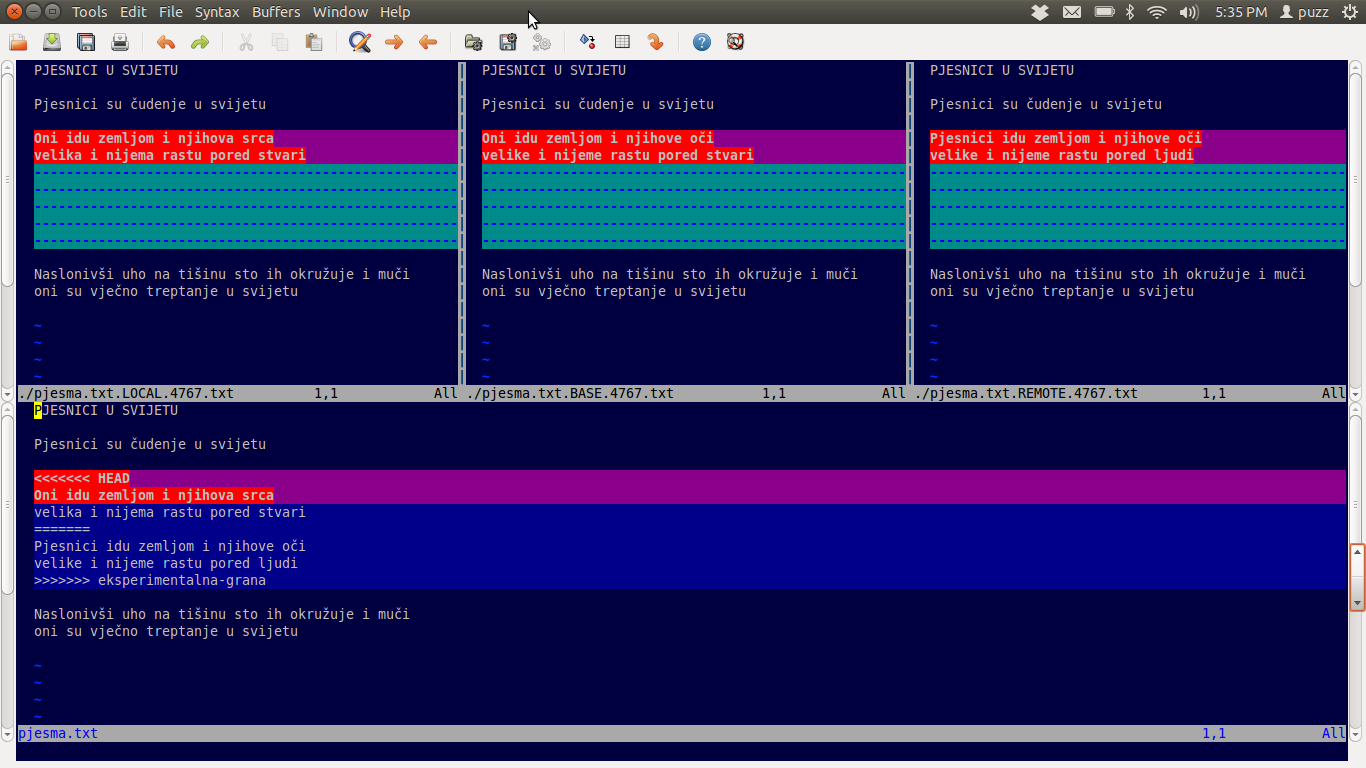
\includegraphics[width=14cm]{images/mergetool.png}

\section*{Merge, branch i povijest projekta}
\addcontentsline{toc}{section}{Merge, branch i povijest projekta}

\section*{Fast forward}
\addcontentsline{toc}{section}{Fast forward}

\section*{Rebase}
\addcontentsline{toc}{section}{Rebase}

% \begin{itemize}
%    \item mergeanje znači mergeanje svih izmjena u povijesti, sve od mjesta gdje su se dvije grane bifucirale
%    \item izuzetak je git cherry-pick (grafovi s obojanim čvorovima)
%    \item --no-ff --no-commit
%    \item rebase
%    \item cherry-pick
%    \item preuzimanje samo jednog fajla iz drugog brancha
%    \item kreiranje privremenog brancha za eksperimentalni merge
% \end{itemize}

%\section*{}
%\addcontentsline{toc}{section}{}


\chapter*{Tagovi}
\addcontentsline{toc}{chapter}{Tagovi}
u
\emph{Tag}, "oznaka", iliti "ključna riječ" je naziv koji je populariziran s dolaskom takozvanim "web 2.0" sajtovima. 
Mnogi ne znaju, ali tagovi su postojali i prije toga. 
Tag je jedan od načina klasifikacije dokumenata.

Standardni način je hijerarhijsko klasifikaciranje.
Po njemu, sve ono što kategoriziramo mora biti u nekoj kategoriji.
Svaka kategorija može imati podkategorije i svaka kategorija može imati najviše jednu nadkategoriju.
Tako klasificiramo životinje, biljke, knjige u knjižnici.
Dakle, postoji "stablo" kategorija i samo jedan čvor može biti "korijen" tog stabla.

Za razliku od toga \emph{tag}iranje je slobodnije.
\emph{Tag}irati možete bilo što i stvari koje \emph{tag}iramo mogu imati proizvoljan broj \emph{tag}ova.
Kad bi u knjižnicama tako označavali knjige, onda one na policama ne bi bilo podijeljene po kategorijama.
Sve bi bile poredane po nekom proizvoljnom redosljedu (na primjer, vremenu kako su stizale u knjižicu), a neki \emph{software} bi za svaku pamtio:

\begin{itemize}
	\item Ključne riječi (iliti \emph{tag}ovi). Na primjer, za neki roman s Sherlockom Holmesom kao glavnim likom, to bi bili "ubojstvo", "krimić", "detektiv", "engleski", "sherlock\_homes", "watson", \dots
	\item Nekakav identifikator knjige (vjerojano ISBN).
	\item Mjesto gdje se knjiga nalazi.
\end{itemize}

Kad bi pretraživali knjige, otišli bi na računalo i utipkali "krimić" i "detektiv" i on bi nam izbacio sve knjige koje imaju oba ta \emph{tag}a.
Tu ne bi bili samo romani Artura Conana Doylea, našli bi se i romani Agathe Christie i mnogih drugih. 
Što više \emph{tag}ova zadamo, to će rezultati pretraživanja biti više specifični.
Uz svaku knjigu bi pisalo na kojoj točno polici se ona nalazi.

Kako mi ovdje radimo s poviješću projekata pa ćemo to i \emph{tag}irati.
Malo preciznije, \emph{tag}irati ćemo čvorove našeg grafa povijesti projekta - \emph{commit}ove.
Postoji samo jedna razlika, \emph{tag} ovdje mora biti jedinstven.
Dakle, ako smo neki tag iskoristili za jedan \emph{commit} onda niti jedan drugi ne smije imati taj isti \emph{tag}.

Kao što znamo, u gitu svaki \emph{commit} ima neki svoj identifikator. 
To je string od 40 znamenaka.
Međutim, taj string je nama ljudima besmislen.

Nama su smisleni komentari uz kod, međutim, ovi \textbf{komentari nisu jedinstveni}.
Projekt možemo pretraživati po riječima iz komentara, ali nema smisla od gita tražiti "Daj mi stanje projekta kakvo je bilo u trenutku kad je komentar \emph{commit} a bio 'Ispravljen bug s izračunom kamate'".
Jer, moglo se desiti da smo imali dva (ili više) \emph{commit}a s komentarom "Ispravljen bug s izračunom kamate".

Sjećate li se priče o verzioniranju koda?
Bilo je riječi o primjeru programera koji radi na programu i izdaje verzije \verb+1.0+, \verb+1.1+, \verb+2.0+, \verb+2.1+\dots svoje aplikacije:

\input{graphs/linearni_model_2}

\dots{}e pa, \emph{tag}ovi bi ovdje bili \verb+1.0+, \verb+1.1+, \verb+2.0+ i \verb+2.1+.

Dakle, \emph{tag} nije ništa drugo nego neki kratki naziv za određeni \emph{commit}, odnosno stanje projekta u nekom trenutku njegove povijesti.

Rad s \emph{tag}ovima je jednostavan; s \verb+git tag+ ćete dobiti spisak svih tretnuno definiranih:

\input{git_output/git_tag}

S \verb+git tag <naziv_taga>+ dodajete novi tag:

\gitoutputcommand{git tag tesni-tag}

\dots{}dok s \verb+git tag -d <naziv_taga>+ brišete neki od postojećih tagova:

\gitoutputcommand{git tag -d testni-tag}

Rad s tagovima je jednostavan, a ima samo jedna komplikacija koja se može dogoditi u radu s udaljenim projektima, no o tome ćemo malo kasnije.

\chapter*{Ispod haube}
\addcontentsline{toc}{chapter}{Ispod haube}

\section*{Kako biste vi\dots}
\addcontentsline{toc}{section}{Kako biste vi\dots}

Da kojim slučajem danas morate dizajnirati i implementirati sustav za verzioniranje koda, kako biste to napravili?
Kako biste čuvali povijest svake datoteke?

Prije nego što ste počeli koristiti takve sustave, vjerojatno ste radili sljedeće: kad bi zaključili da ste došli do nekog važnog stanja u projektu, kopirali bi cijeli projekt u direktorij naziva \verb+projekt_backup+ ili \verb+projekt_2012_04_05+ ili neko drugo slično ime.
Rezultat je da ste imali gomilu sličnih "backup" projekata.
Svaki direktorij predstavlja neko stanje projekta (dakle to je \emph{commit}.
I to je nekakvo verzioniranje koda, no puno toga nedostaje.

Na primjer, nemate komentare uz \emph{commit}ove, ali to bi se moglo srediti tako da u svaki direktorij spremite datoteku naziva \verb+komentar.txt+.
Nemate niti nekakav graf, odnosno redosljed kako su direktorij nastajali jedan iz drugog.
I to bi se moglo riješit tako da u svakom direktoriju u nekoj posebnoj datoteci, npr. \verb+parents+ nabrojite nazive direktorija koji su "roditelji" trenutnom direktoriju.

No, sve je to prilično neefikasno što se tiče diskovnog prostora. 
Imate li u repozitoriju jednu datoteku veličine 100 kilobajta koju \emph{nikad} ne mijenjate, njena kopija će opet zauzimati 100 kilobajta u svakoj kopiji projekta.
To je gnjavaža.

Zato bi možda bilo bolje da umjesto \textbf{kopije direktorija} za \emph{commit} napravimo novi u kojeg ćemo staviti \textbf{samo one datoteke koje su izmijenjene}.
Zahtijevalo bi malo više posla jer morate točno znati koje su datoteke izmijenjene, ali i to se može riješiti.
Mogli bi napraviti neku jednostavno \emph{shell} skriptu koja će to napraviti a nas. 

S time bi se problem diskovnog prostora drastično smanjio. 
Rezultat bi mogli još malo poboljšati tako da datoteke kompresiramo.

Još jedna varijanta bi bila da ne čuvate izmijenjene datoteke, nego samo izmijenjene linije koda.
Tako bi, vaše datoteke, umjesto cijelog sadržaja imale nešto tipa "Peta linija izmijenjena iz 'def suma\_brojeva()' u 'def zbroj\_brojeva()'".
To su takozvane "delte".
Još jedna varijanta bi bila da ne radite kopije direktorija, nego sve snimate u jednom tako da za svaku datoteku čuvate originalnu verziju i nakon toga (u istoj datoteci) dodajete delte.
Onda će vam trebati nekakav pomoćni programčić kako iz povijesti izvući zadnju verziju bilo koje datoteke, jer on mora izračunati sve delte od početne verzije.

Sve te varijante imaju jedan suptilni, ali neugodan, problem.
Problem konzistencije.

Vratimo se na trenutak na ideju s kopiranjem direktorija sa izmijenjenim datotekama.
Ako svaki direktorij sadrži samo izmijenjene datoteke, onda prvi direktorij mora sadržavati \emph{sve} datoteke.
Pretpostavite da imate jednu datoteku koja nije nikad izmijenjena od prve do zadnje verzije. 
Ona će se nalaziti samo u prvom (originalnom) direktoriju.

Što ako neki zlonamjernik upadne u vaš sustav i izmijeni takvu datoteku?
Razmislimo malo, on je upravo izmijenio ne samo početno stanje takve datoteke nego je \textbf{promijenio cijelu njenu povijest}!
Kad bi vi svoj sustav pitali "daj mi zadnju verziju projekta", on bi protrčao kroz sva stanja projekta i dao bi vam hakerovu varijantu.
Jeste li sigurni da bi primijetili podvaljenu datoteku?

Riješenje je da je vaš sustav nekako dizajniran tako da sam prepoznaje takve izmijenjene datoteke. 
Odnosno, da je tako dizajniran da, ako bilo tko promijeni nešto u povijesti -- sam sustav prepozna da nešto s njime ne valja.
To se može na sljedeći način: neka jedinstveni identifikator svakog \emph{commit}a bude neki podatak koji je \textbf{izračunat} iz sadržaja i koji jedinstveno određuje sadržaj.
Takav jedinstveni identifikator će se nalaziti u grafu projekta, i sljedeći \emph{commit}ovi će znati da im je on prethodnik.

Ukoliko bilo tko promijeni sadržaj nekog \emph{commit}a, onda on više neće odgovarati tom identifikatoru.
Promijeni li i identifikator, onda graf više neće biti konzistentan -- sljedeći \emph{commit} će sadržavati identifikator koji više ne postoji.
Dakle, haker bi trebao promijeniti sve \emph{commit}ove do zadnjeg. 
U biti, trebao bi promijeniti previše stvari da bi mu cijeli poduhvat mogao proći nezapaženo.

Još ako je naš sustav distribuiran (dakle i drugi korisnici imaju povijest cijelog projekta) onda mu je još teže -- jer tu radnju mora ponoviti na računalima svih ljudi koji imaju kopije.
S distribuiranim sustavima, nitko nikad niti ne zna tko sve ima kopije.

Nakon ovog početnog razmatranja, idemo pogledati koje od tih ideja su programeri gita uzeli kad su krenuli dizajnirati svoj sustav.
Krećimo s problemom konzistentnosti.

\section*{SHA1}
\addcontentsline{toc}{section}{SHA1}

Znate li malo matematike čuli ste za jednosmerne funkcije.
Ako i niste, nije bitno. 
To su funkcije koje je lako izračunati, ali je izuzetno teško iz rezultata zaključiti kakav je mogao biti početni argument.
Takve su, na primjer, \emph{hash} funkcije, a jedna od njih je SHA1.

SHA1 kao argument uzima string i iz njega izračunava drugi string duljine 40 znakova.
Primjer takvog stringa je \verb+974ef0ad8351ba7b4d402b8ae3942c96d667e199+.

Izgleda poznato?

SHA1 ima sljedeća svojstva:

\begin{itemize}
	\item \emph{Nije} jedinstvena. Dakle, sigurno postoje različiti ulazni stringovi koji daju isti rezultat, no \textbf{praktički ih je nemoguće naći}\footnote{Ovdje treba napomenuti kako SHA1 nije \emph{potpuno} siguran. Ukoliko se nađe algoritam s kojime je moguće naći različite stringove za prizvoljne SHA1 stringove, onda on prestaje biti jednosmjerna funkcija. I tada cijela sigurnost potencijalno pada u vodu, jer netko može podvaliti drukčiji string u povijest za isti SHA1 string. Postoje istraživanja koja naznačuju da se to može. Moguće je da će git u budućnosti preći na SHA-256.}. 
	\item Kad dobijete rezultat funkcije (npr. \verb+974ef0ad8351ba7b4d402b8ae3942c96d667e199+) is njega je \textbf{praktički nemoguće izračunati string iz kojeg je nastala}.
\end{itemize}

Takvih $40-$znamenkastih stringova ćete vidjeti cijelu gomilu u \verb+.git+ direktoriju.

Git nije ništa drugo nego graf SHA1 stringova, od kojih svaki jedinstveno identificira neko stanje projekta \textbf{i izračunati su iz tog stanja}.
Osim SHA1 identifikatora git uz svaki \emph{commit} čuva i neke metapodatke kao, na primjer:

\begin{itemize}
	\item Datum i vrijeme kad je nastao.
	\item Komentar
	\item SHA1 \emph{commit}a koji mu je prethodio
	\item SHA1 \emph{commit}a iz kojeg su preuzete izmjene za \emph{merge} (\textbf{ako} je taj \emph{commit} rezultat \emph{merge}a).
	\item \dots
\end{itemize}

Buduću da je svaki \emph{commit} SHA1 sadržaja projekta u nekom trenutku, kad bi netko htio neopaženo promijeniti povijest projekta, morao bi promijeniti i njegov SHA1 identifikator.
No, onda mora promijeniti i SHA1 njegovog sljedbenika, i sljedbenika njegovog sljedbenika, i\dots

\section*{Grane}
\addcontentsline{toc}{section}{Grane}

Razmislimo o još jednom detalju, uz poznati graf:

\input{graphs/primjer_s_imenovanim_granama_i_spajanjima}

Graf kao ovaj gore matematičari zovu usmjereni graf jer su veze između čvorova usmjerene: $\vec{ab}$, $\vec{bc}$, itd.
Znamo već da svaki čvor tov grafa predstavlja stanje nekog projekta, a svaka strelica neku izmjenu u novo stanje.

Sad kad znamo ovo malo pozadine oko toga kako git interno pamti podatke, gornji graf bi mogli prikazati i ovako:

\input{graphs/primjer_s_imenovanim_granama_i_spajanjima_suprotne_strelice}

Sve strelice su ovdje usmjerene suprotno negoli u grafovima kakve smo do sada imali.
Naime, čvor \emph g ima referencu na na \emph g, \emph g ima reference na \emph f i na \emph q, itd.
Uočite da nam uopće nije potrebno znati da se grana \verb+novi-feature+ sastoji od \emph x, \emph y, \emph z, \emph q i \emph w.
Dovoljan nam je $w$.
Iz njega možemo, prateći reference "unazad" (suprotno od kronološkog reda nastajanja) doći sve do mjesta gdje je grana nastala.

Zato gitu interno grane i nisu ništa drugo neki reference na njihove zadnje \emph{commit}ove.

\section*{.git direktorij}
\addcontentsline{toc}{section}{.git direktorij}

Pogledajmo, na trenutak, onaj \verb+.git+ direktorij. 
Vjerojatno ste to već učinili, i vjerojatno ste otkrili da je njegov sadržaj otprilike ovakav:

\input{git_output/dot_git_folder}

Samo ukratko ćemo ovdje opisati neke važne dijelove: \verb+.git/objects+, \verb+.git/refs+, \verb+HEAD+ i \verb+.git/hooks+

\subsection*{.git/objects}
\addcontentsline{toc}{subsection}{.git/objects}

\input{git_output/git_objects}

\subsection*{.git/refs}
\addcontentsline{toc}{subsection}{.git/refs}

\input{git_output/find_dot_git_refs}

\subsection*{HEAD}
\addcontentsline{toc}{subsection}{HEAD}

\subsection*{.git/hooks}
\addcontentsline{toc}{subsection}{.git/hooks}

%\section*{}
%\addcontentsline{toc}{section}{}


\chapter*{Povijest}
\addcontentsline{toc}{chapter}{Povijest}

Već smo se poznali s naredbom \verb+git log+ s kojom se može vidjeti povijest \emph{commit}ova grane u kojoj se trenutno nalazimo, no ona zasigurno nije dovoljna za proučavanje povijesti projekta.
Posebno s git projektima, čija povijest zna biti dosta kompleksna (puno grana, \emph{merge}anja, isl.).

Sigurno će vam se ponekad desiti da želite vidjeti koje se se izmjene desile između predzadnjeg i pred-predzanjeg \emph{commit}a ili da vratite neku neku datoteku u stanje kakvo je bilo prije mjesec dana ili da proučite tko je zadnji napravio izmjenu na trinaestoj liniji nekog programa ili tko je prvi uveo funkciju koja se naziva \verb+get_image_x_xizse+ u projektu\dots 
Čak i ako vam se neki od navedenih scenarija, vjerujte mi -- trebati će vam.

U ovom poglavlju ćemo proći samo neke od često korištenih varijanti naredbi za proučavanje povijesti projekta.

\section*{Diff}
\addcontentsline{toc}{section}{Diff}

Važna naredba je i \verb+git diff+. 
S njome provjeravate razlike između dva \emph{commit}a.
Na primjer:

\gitoutputcommand{git diff master tesna-grana}

\dots{}će nam ispisati razliku između dvije grane. Pripazite, jer redosljed je ovdje bitan.
Ukoliko isprobate s:

\gitoutputcommand{git diff tesna-grana master}

\dots{}dobiti ćete suprotan ispis. 
Ako ste u \verb+testna-grana+ jedan redak dodali -- u jednom slučaju će \verb+diff+ ispisati da ste ga dodali, a u drugom oduzeli.

Želite li provjeriti koje su izmjene dogodile između predzadnjeg i pred-predzadnjeg commita:

\gitoutputcommand{git diff HEAD\textasciitilde{}2 HEAD\textasciitilde{}1}

\dots{}ili između pred-predzadnjeg i sadašnjeg:

\gitoutputcommand{git diff HEAD\textasciitilde{}2}

\dots{}ili izmjene između \verb+974ef0ad8351ba7b4d402b8ae3942c96d667e199+ i \verb+testna-grana+:

\gitoutputcommand{git diff 974ef testna-grana}

\section*{Log}
\addcontentsline{toc}{section}{Log}

Standardno s \verb+git log <naziv_grane>+ će vam ispisati povijest te grane.
Sad kad znamo da je grana u biti samo referenca na zadnji \emph{commit}, znamo i da bi bilo preciznije kazati da je ispravna sintaksa \verb+git log <referenca_na_commit>+.
Za git nije previše bitno jeste li mu dali naziv grane ili referencu na \emph{commit}, on će jednostavno krenuti "unazad" po grafu i dati vam povijest koju na taj način nađe.
Pa tako, ako želimo povijest trenutne grane, ali bez zadnjih pet unosa, pitati ćemo jednostavno:

\gitoutputcommand{git log HEAD\textasciitilde{}5}

Ili, ako želimo povijest grane \verb+testna-grana+ bez zadnjih 10 unosa:

\gitoutputcommand{git log testna-grana\textasciitilde{}10}

Želimo li povijest sa \emph{samo} nekoliko zadjnih unosa, koristimo \verb+git log -n+ sintaksu:

\gitoutputcommand{git log -10 testna-grana}

\dots{}ili, ako to želimo za trenutnu granu, jednostavno:

\gitoutputcommand{git log -10}

\subsection*{Pretraživanje povijesti}
\addcontentsline{toc}{subsection}{Pretraživanje povijesti}

Vrlo često će vam se dogoditi da tražite neki \emph{commit} iz povijesti.
Ovdje ćemo proći samo dva najčešća slučaja.
Prvi je kad pretražujete prema tekstu \emph{commit}a, tada se koristi \verb+git log --grep=<regularni_izraz>+.
Na primjer, tražim li sve \emph{commit}ove koji u sebi sadrže riječ \verb+graph+:

\gitoutputcommand{git log --grep=graph}

Drugi česti scenarij je odgovor na pitanje "Kad se u kodu prvi put spomenuo string 'x'"? Tada se koristi \verb+git log -S<string>+.
Recimo da tražite tko je prvi napisao funkciju \verb+get_image_width+:

\gitoutputcommand{git log -Sget\_image\_width}

Treba li pretraživati za string s razmacima:

\gitoutputcommand{git log -S"get image width"}

Zapamtite, ovo će vam samo naći \emph{commit}ove.
Kad ih nađete, sigurno ćete htjeti pogledati koje su točno bile izmjene.
Ako vam pretraživanje nađe da je \emph{commit} \verb+76cf802d23834bc74473370ca81993c5b07c2e35+, detalji izmjena koje su se njime dogodile su:

\gitoutputcommand{git diff 76cf8 76cf8\textasciitilde{}1}

\section*{Blame}
\addcontentsline{toc}{section}{Blame}

S \verb+git blame <datoteka>+ ćete dobiti ispis datoteke s detaljima o tome \textbf{tko}, \textbf{kad} i u \textbf{kojeg \emph{commit}u} je napravio svaku liniju u toj datoteci i \textbf{iz koje datoteke} je ta izmjena došla ovdje:

\input{git_output/git_blame}

\section*{Whatchanged}
\addcontentsline{toc}{section}{Whatchanged}

Naredba \verb+git whatchanged+ je vrlo slična \verb+git log+, jedino što uz svaki \emph{commit} ispisuje i spisak svih datoteka koje su se tada promijenile:

\input{git_output/git_whatchanged}

\section*{Preuzimanje datoteke iz povijesti}
\addcontentsline{toc}{section}{Preuzimanje datoteke iz povijesti}

\section*{Gitk}
\addcontentsline{toc}{section}{Gitk}

\section*{Reset}
\addcontentsline{toc}{section}{Reset}

\section*{Revert}
\addcontentsline{toc}{section}{Revert}

%\section*{}
%\addcontentsline{toc}{section}{}

\chapter*{Udaljeni repozitoriji}
\addcontentsline{toc}{chapter}{Udaljeni repozitoriji}

Sve ono što smo do sada proučavali smo radili isključivo na lokalnom repozitoriju.
Samo smo spomenuli da je git distribuirani sustav za verzioniranje koda, složiti ćete se da je već krajnje vrijeme da krenemo pomalo obrađivati interakciju s udaljenim repozitorijima.

Postoji puno scenarija kako može funkcionirati ta interakcija.
Koncentrirajmo se sada na sam trenutak kad repozitorij "dođe" ili "nastane" na našem lokalnom računalu.
Moguće je da smo ga stvorili od nule s \verb+git init+, na način kako smo to radili do sada i onda, na neki način, "poslali" na neku udaljenu lokaciju.
Ili smo takav repozitorij ponudili drugim ljudima da ga preuzmu (kloniraju).

No, moguće je i da smo saznali za neki već postojeći repozitorij, negdje na internetu, i sad želimo i mi preuzeti taj kod.
Bilo da je to zato što želimo pomoći u razvoju ili samo proučiti nečiji kod.
Krenimo s prvim tipičnim scenarijem\dots

\section*{Naziv i adresa repozitorija}
\addcontentsline{toc}{section}{Naziv i adresa repozitorija}

Prvu stvar koju ćemo obraditi je kloniranje udaljenog repozitorija.
No, ima prije toga jedna sitnica koju trebamo znati.
Svaki udaljeni repozitorij s kojime će git "komunicirati" mora imati svoju adresu.

Na primjer, ova knjiga "postoji" na \verb+git://github.com/tkrajina/uvod-u-git.git+, i to je jedna njega andresa.
Github\footnote{Web servis koji omogućava da držite svoje git repozitorije} omogućava da se istim repozitoriju pristupi i preko \\ \verb+https://tkrajina@github.com/tkrajina/uvod-u-git.git+.
Osim na Githubu, ona živi i na mom lokalnom računalu i u tom slučaju je njena adresa \verb+/home/puzz/projects/uvod-u-git+ (direktorij u kojemu se nalazi).

Nadalje, svaki udaljeni repozitorij ima i svoje kratko ime.
Nešto kao: \verb+origin+ ili \\ \verb+vanjin-repozitorij+ ili \verb+slobodan+ ili \verb+dalenov-repo+.
Nazivi su vaš slobodan izbor. 
Tako, ako vas četvero radi na istom projektu, njihove udaljene repozitorije možete nazvati \verb+marina+, \verb+ivan+, \verb+karla+.
I sa svakim od njih možete imati nekakvu vrstu interakcije. 
Na neke ćete slati svoje izmjene (ako imate ovlasti), a s nekih ćete izmjene preuzimati u svoj repozitorij.

\section*{Kloniranje repozitorija}
\addcontentsline{toc}{section}{Kloniranje repozitorija}

Kloniranje je postupak kojim kopiramo cijeli repozitorij na nekoj udaljenoj lokaciji na naše lokalno računalo, a da bi onda s njime dalje nastavili raditi.
U stvari, kopirati repozitorij je jednostavno, dovoljno je u neki direktorij kopirati \verb+.git+ direktorij drugog repzitorija i onda u njemu napraviti \verb+git checkout HEAD+.

Kloniranje je za nijansu drukčije.
Recimo to ovako, \textbf{kloniranje je kopiranje udaljenog repozitorija, ali tako da novi (lokalni) repozitorij ostaje "svjestan" da je on kopija nekog udaljenog repozitorija}.

Postupak je jednostavan, ako znamo adresu (a moramo znati), onda\dots

\input{git_output/git_clone}

\dots{}\textbf{kopira cijeli projekt, zajedno sa cijelom poviješću} na naše računalo.
I to u direktorij \verb+uvod-u-git+.
Sad tu možemo gledati povijest, granati, \emph{commit}ati, \dots Raditi što god nas je volja s tim projektom.

Jasno, ne može bilo tko kasnije svoje izmjene poslati nazad na originalnu lokaciju. 
Za to moramo imati ovlasti, ili moramo vlasnika tog repozitorija pitati je li voljan naše izmjene preuzeti kod sebe.
O tome malo kasnije.

E, i još nešto. Sjećate se kad sam napisao da su nazivi udaljenih repozitorija vaš slobodan izbor.
Nisam baš bio $100\%$ iskren. 
Kloniranje je izuzetak.
Ukoliko kloniramo udaljeni repozitorij, on se za nas zove \verb+origin+.
Ostali repozitoriji koje ćemo dodavati mogu imati nazive kakve god želimo.

\subsection*{Struktura kloniranog repozitorija}
\addcontentsline{toc}{subsection}{Struktura kloniranog repozitorija}

Od trenutka kad smo klonirali svoj repozitorij pa na dalje -- za nas postoje \textbf{dva repozitorija}.
Možda negdje na svijetu postoji još netko tko je klonirao taj isti repozitorij i na njemu nešto radi (a da mi o tome ništa ne znamo).
No, naš dio svijeta su samo ova dva s kojima direktno imamo posla. 
Jedan je udaljeno kojeg smo klonirali, a drugi je lokalni koji se nalazi pred nama.

Prije negoli počnemo s pričom o tome kako slati ili primati izmjene iz jednog repozitorija u drugi, trebamo nakratko spomenuti kakva je točno struktura lokalnog repozitorija.
Već znamo za naredbu \verb+git branch+, koja nam ispisuje spisak svih grana na našem repozitoriju.
No, sad imamo posla i sa udaljenim repozitorijem -- njega smo klonirali.

S \verb+git branch -a+ ispisujemo \textbf{sve grane koje su nam trenutno dostupne u lokalnom rpeozitoriju}.
Naime, kad smo klonirali repozitorij -- postale su nam dostupne i grane udaljenog repozitorija:

\input{git_output/git_branch_all_1}

Novost ovdje je \verb+remotes/origin/master+.
Prvo, ovo \verb+remotes/+ znači da, iako toj grani imamo pristup na lokalnom repozitoriju, ona je \textbf{samo kopija grane} \verb+master+ \textbf{u repozitoriju} \verb+origin+.
Takve kopije udaljenih repozitorija ćemo uvijek označavati s \\ \verb+<naziv_repozitorija>/<naziv_grane>+.
Konkretno, ovdje je to \verb+origin/master+.

Dakle, grafički bi to mogli prikazati ovako:

\input{graphs/origin_master}

Imamo dva repozitorija, lokalni i udaljeni.
Udaljeni ima samo granu \verb+master+, a lokalni ima dvije kopije te grane. 
U lokalnom \verb+master+ ćemo mi \emph{commit}ati naše izmjene, a u \verb+origin/master+ se nalazi kopija udaljenog \verb+origin/master+ u koju \textbf{nećemo} \emph{commit}ati.
Ovaj \verb+origin/master+ ćemo, s vremenena na vrijeme, osvježavati tako da imamo ažurno stanje udaljenog repozitorija.

Ako vam ovo zvuči zbunjujuće, ništa čudno.
No, sve će sjesti na svoje mjesto kad to počnete koristiti.

\TODO: \verb+checkout origin/master+, log, diff, merge

\subsection*{Djelomično kloniranje povijesti repozitorija}
\addcontentsline{toc}{subsection}{Djelomično kloniranje povijesti repozitorija}

Našli ste na internetu neki zanimljiv projekt i njegov git repozitorij i htjeli bi ga skinuti i proučiti njegov kod. 
Ništa lakše; \verb+git clone ...+.

E, ali\dots
Tu imamo mali problem.
Git repozitorij sadrži cijelu povijest projekta. 
To znači da sadrži sve \emph{commit}ove koje su radili programeri i koji mogu sezati i preko deset godina unazad.
I zato \verb+git clone+ ponekad može potrajati dosta dugo. 
Posebno ako imate sporu vezu.

No, postoji trik.
Želimo li skinuti projekt samo zato da bi pogledali njegov kod a ne zanima nas cijela njegova povijest -- moguće je klonirati samo nekoliko njegovih zadnjih \emph{commit}ova s:

\gitoutputcommand{git clone --depth 5 --no-hardlinks git://github.com/tkrajina/uvod-u-git.git}

To će biti puno brže, no nećete imati pristup cijeloj povijesti, nego samo zadnjih $5$ \emph{commit}ova.

\TODO: Ograničenja takvog kloniranja


\section*{Fetch}
\addcontentsline{toc}{section}{Fetch}

Što ako je vlasnik udaljenog repozitorija \emph{commit}ao u svoj \verb+master+.
Stanje je sad ovakvo:

\input{graphs/origin_master_2}

Naš, lokalni, \verb+master+ je radna verzija s kojom ćemo mi raditi -- tj. na koju ćemo \emph{commit}ati.
\verb+origin/master+ bi trebao biti lokalna kopija udaljenog \verb+master+, međutim -- ona se ne ažurira automatski.
To što je vlasnik udaljenog repozitorija dodao dva \emph{commit}a ($e$ i $f$) ne znači da će naš repozitorij nekom čarolijom to odmah saznati.

Git je zamišljen kao sustav koji ne zahtijeva stalni pristup internetu.
U većini operacija -- \textbf{od nas se očekuje da iniciramo interakciju s drugim repozitorijima}.
Bez da mi pokrenemo neku radnju, git neće nikad kontaktirati udaljene repozitorije.
Isto tako u drugom smjeru -- ni u jednoj situaciji neki drugi repozitorij ne može inicirati neki proces na našem repozitoriju.
Najviše što što vlasnik udaljenog repozitorija može napraviti je da nas \textbf{zamoli} da mi napravimo neku interakciju s njegovim repozitorijem.

Kao što smo mi inicirali kloniranje, tako i mi moramo inicirati ažuriranje grane \verb+origin/master+.
To se radi s \verb+git fetch+:

\input{git_output/git_fetch}

Nakon toga, stanje naših repozitorija je:

\input{graphs/origin_master_3}

Dakle, \verb+origin/master+ je osvježen tako da mu je stanje isto kao i \verb+master+ udaljenog repozitorija.

S \verb+origin/master+ možemo raditi skoro sve kao i s ostalim lokalnim granama.
Možemo, na primjer, pogledati njegovu povijest s:

\gitoutputcommand{git log origin/master}

Možemo pogledati razlike između njega i naše trenutne grane:

\gitoutputcommand{git diff origin/master}

Možemo se prebaciti da \verb+origin/master+, ali\dots

\input{git_output/git_checkout_origin_master}

Git nam ovdje dopušta prebacivanje na \verb+origin/master+, ali nam jasno daje do znanja da je ta grana ipak po nečemu posebna.
Kao što već znamo, ona nije zamišljena da s njome radimo direktno.
Nju možemo samo osvježavati stanjem iz udaljenog repozitorija.
U \verb+origin/master+ ne smijemo \emph{commit}ati.

Ima, ipak, jedna radnja koju trebamo raditi s \verb+origin/master+, a to je da izmjene iz nje preuzimamo u naš lokalni \verb+master+.
Prebacimo se na njega s \verb+git checkout master+ i\dots{}

\gitoutputcommand{git merge origin/master}

\dots{}i sad je stanje:

\input{graphs/origin_master_4}

I sad smo tek u \verb+master+ dobili stanje udaljenog \verb+master+.
Općenito, to je postupak kojeg ćemo često ponavljati:

\gitoutputcommand{git fetch}

\dots{}da bismo osvježili svoj lokalni \verb+origin/master+.
Sad tu možemo malo proučiti njegovu povijest i izmjene koje uvodi u povijest.
I onda\dots

\gitoutputcommand{git merge origin/master}

\dots{}da bi te izmjene unijeli u naš lokalni repozitorij.

Malo složeniji scenarij je sljedeći -- recimo da smo nakon\dots{}

\input{graphs/origin_master_2}

\dots{}mi \emph{commit}ali u naš lokalni repozitorij svoje izmjene. Recimo da su to $x$ i $y$:

\input{graphs/origin_master_2_2}

Nakon \verb+git fetch+, stanje je:

\input{graphs/origin_master_2_3}

Sad \verb+origin/master+ nakon $e$ ima $f$ i $g$, a \verb+master+ nakon $e$ ima $x$ i $y$.
U biti je to kao da imamom dvije grane koje su nastale nakon $e$. Jedna ima $f$ i $g$, a druga $x$ i $y$.
Ovo je, u biti, najobičniji \emph{merge} (koji će, eventualno, imati i neke konflikte. No, to već znamo riješiti).
Rezultat \emph{merge}a je novi čvor $z$:

\input{graphs/origin_master_2_4}

\section*{Pull}
\addcontentsline{toc}{section}{Pull}

U prethodnom poglavlju smo opisali da je tipični redosljed naredbi koje ćemo izvršiti svaki put kad želimo preuzeti izmjene iz udaljenog repozitorija:

\gitoutputcommand{git fetch\\git merge origin/master}

Obično ćemo nakon \verb+git fetch+ malo pogledati koje izmjene su došle s udaljenog repozitorija, no u konačnici ćemo ove dvije naredbe htjeti skoro uvijek izvršiti.

Zbog toga postoji "kratica" koja je ekvivalentna toj kombinaciji:

\gitoutputcommand{git pull}

\verb+git pull+ je upravo kombinacija \verb+git fetch+ i \verb+git merge origin/master+.

\section*{Push}
\addcontentsline{toc}{section}{Push}

Sve što smo do sada radili s gitom su bile radnje koje smo mi radili na našem lokalnom repozitoriju.
Čak i kloniranje je nešto što mi iniciramo i ničim nismo promijenili udaljeni repozitorij.
Krećemo sad na prvu (i ovdje jedinu) radnju s kojom aktivno mijenjamo neki udaljeni repozitorij.

Uzmimo, kao prvo, najjednostavniji mogući scenarij.
Klonirali smo repozitorij i stanje je, naravno:

\input{graphs/push_1}

Nakon toga smo \emph{commit}ali par izmjena\dots

\input{graphs/push_2}

\dots{}i sad bi htjeli te izmjene "prebaciti" na udaljeni repozitorij.
Prvo i osnovno što nam treba svima biti jasno -- "prebacivanje" naših lokalnih izmjena na udaljeni repozitorij ovisi o tome imate li ovlasti za to ili ne.
Udaljeni repozitorij mora biti tako konfiguriran da biste to mogli činiti.
Ukoliko nemate ovlasti, sve što možete napraviti je zamoliti njegovog vlasnika da pogleda vaše izmjene ($f$ i $g$) i da ih preuzme kod sebe.

Ukoliko, ipak, imate ovlasti, onda je ono što trebate napraviti:

\input{git_output/git_push_origin_master}

Stanje će sad biti:

\input{graphs/push_3}

Ovo je bio jednostavni scenarij u kojem smo u našem \verb+master+ \emph{commit}ali, ali u udaljenom \verb+master+ se nije ništa događalo.
Što da nije tako?
Dakle, dok smo mi radili na $e$ i $f$, vlasnik udaljenog repozitorija je \emph{commit}ao svoje $x$ i $y$:

\input{graphs/push_2_1}

\section*{Rad s granama}
\addcontentsline{toc}{section}{Rad s granama}

\section*{Udaljeni repozitoriji}
\addcontentsline{toc}{section}{Udaljeni repozitoriji}

\subsection*{Dodavanje i brisanje udaljenih repozitorija}
\addcontentsline{toc}{subsection}{Dodavanje i brisanje udaljenih repozitorija}

\subsection*{Rad s udaljenim repozitorijima}
\addcontentsline{toc}{subsection}{Rad s udaljenim repozitorijima}

tagovi, \dots

\TODO "Bare" repozitorij

%\section*{}
%\addcontentsline{toc}{section}{}


% TODO
%\chapter*{Podstabla}
\addcontentsline{toc}{chapter}{Podstabla}

Kad imamo dva projekta, svi mi programeri prirodno težimo k tome da izvučemo zajednički kod u neki treći (\emph{utility}) projekt.
Tako da isti kod koristimo na više mjesta, a ne da svaki put izmišljamo toplu vodu.
Postoje mnogi načini kako se takvi projekti organiziraju.

Na primjer, ako radimo u javi, onda možete takve \emph{utility} projekte upakirati u \verb+.jar+ datoteke i koristiti ih u ostalim projektima.
U \emph{IDE}ovima\footnote{Integrated development environment -- alati kao Eclipse, NetBeans, Idea, Visual studio, \dots} možemo imati projekte koji referenciraju druge projekte, i sl.

Git nudi jednu sličnu mogućnost koju možemo koristiti, a to su \emph{submodul}i.

Git \emph{submodul} je \textbf{referenca na točno određeni \emph{commit} nekog drugog projekta na nekom mjestu u direktoriju našeg projekta}.
I onda uz pomoć git-a možemo klonirati cijeli pomoćni projekt i postaviti ga na taj \emph{commit}.

U stvari\dots Zaboravite zadnje dvije rečenice. Idemo ispočetka!

Taman napisah gornje dvije rečenica, kad mi je došla vijest da git u zadnjoj verziji ima jedan noviji i bolji mehanizam koji će (nadam se) u potpunosti zamijeniti \emph{submodul}e.

\TODO Dodavanje

\TODO Kako je konfigurirano

\TODO Brisanje

\TODO Izmjene

\TODO Postupak kad kloniramo projekt koji ima submodule

%\section*{}
%\addcontentsline{toc}{section}{}


\chapter*{"Higijena" repozitorija}
\addcontentsline{toc}{chapter}{"Higijena" repozitorija}

Naš repozitorij je naš životni prostor i s njime živimo dio dana.
Kao što se trudimo držati stan urednim, tako bi trebalo i s našim virtualnim prostorima.
Preko tjedna, kad rano ujutro odlazimo na posao i vraćamo se kasnije popodne, se ponekad desi da nam se u stanu nagomila robe za pranje.
No, nekoliko puta tjedno treba uzeti pola sata vremena i počistiti nered koji je zaostao.

Tako i s repozitorijem.
Ima nekoliko stvari na koje bi trebali pripaziti.

\subsection*{Grane}
\addcontentsline{toc}{subsection}{Grane}

Nemojte si dopustiti da grane u vašem repozitoriju izgledaju ovako "zbrčkano":

\input{graphs/cirkus}

Iako nam git omogućuje da imamo neograničen broj grana, ljudski um nije sposoban vizualizirati si više od 5-10 njih\footnote{Barem moj nije, ako je vaš izuzetak, preskočite sljedećih nekoliko rečenica. Ili jednostavno zamislite da je umjesto "5-10" pisalo "500-1000".}.
Kako stvaramo nove grane -- dešava se da imamo one u kojima smo počeli neki posao i kasnije odlučili da nam ne treba.
Ili smo napravili posao, \emph{merge}ali u \verb+master+, ali nismo obrisali granu.
Nađemo li se s više od 10-15 grana -- \textbf{sigurno} je dio njih tu samo zato što smo ih zaboravili obrisati.

U svakom slučaju, predlažem vam da svakih par dana pogledate malo po lokalnim (a i udaljenim granama) i provjerite one koje više ne koristite.

Ukoliko nismo sigurni je li nam u nekoj grani ostala možda još kakva izmjena koju treba vratiti u \verb+master+, postupak je sljedeći:

\gitoutputcommand{git checkout neka-grana\\git merge master}

\dots{}da bismo preuzeli sve izmjene iz master, tako da stanje bude ažurno.
I sad\dots

\gitoutputcommand{git diff master}

\dots{}da bismo provjerili koje su točno izmjene ostale.
Ako je prazno -- nema razlika i možemo brisati.
Ako nije -- \textbf{ima} izmjena i sad se sami odlučite jesu li te izmjene nešto važno što ćete nastaviti razvijati ili nešto što možemo zanemariti i obrisati tu granu.

\subsection*{Git gc}
\addcontentsline{toc}{subsection}{Git gc}

Druga stvar koju se preporuča ima veze s onim našim \verb+.git/objects+ direktorijem kojeg smo spominjali u "Ispod haube" poglavlju.
Kao što znamo, svaki \emph{commit} ima svoju referencu i svoj objekt (datoteku) u tom direktoriju.
Kad napravimo \verb+git commit --amend+ -- git stvara \textbf{novi} \emph{commit}.
Nije da on samo izmijeni stari\footnote{Ne bi ni mogao izmijeniti stari, jer ima drukčiji sadržaj i SHA1 bi mu se nužno morao promijeniti.}.

Grafički:

\input{graphs/amend}

Dakle, git interno dodaje \textbf{novi} objekt (\emph{f'}) i na njega pomiče referencu \verb+HEAD+ (koja je do tada gledala na \emph f).
On samo "kaže": Od sada na dalje, zadnji \emph{commit} u ovoj grani više nije \emph f, nego \emph{f'}.

No, sad u git repozitoriju imamo i \emph{commit} \emph f, a i \emph{f'}, ali samo jedan od njih se koristi (\emph{f'}).
Commit \emph f je \textbf{i dalje snimljen u} \verb+.git/object+ \textbf{direktoriju}.
I on se više neće koristiti.
Puno tih \verb+git commit --amend+ posljedično ostavlja puno takvog "smeća" u repozitoriju.

To vrijedi i za neke druge operacije kao brisanje grana ili rebase.
Git to čini da bi tekuće operacije bilo što je brže moguće.
Čišćenje takvog "smeća" (\emph{garbage collection} iliti \emph{gc}) ostavlja za kasnije, a ta radnja nije automatizirana nego se od nas očekuje da ju izvršimo\footnote{Nije automatizirana, ali možemo uvijek sami napraviti neki task koji se izvršava na dnevnoj ili tjednoj bazi, a koji "čisti" sve naše git repozitorije.}.

Naredba je \verb+git gc+:

\input{git_output/git_gc}

\dots{}i nju treba izvršavati s vremena na vrijeme.

Osim \verb+gc+, postoji još nekoliko sličnih naredbi kao \verb+git repack+, \verb+git prune+, no one su manje važne za početnika.
Ako vas zanima -- \verb+git help+ je uvijek na dohvat ruke.

\tocChapter{Česta pitanja}

Jedno je razumijeti naredbe i terminologiju gita, a potpuno drugo je imati iskustvo u radu s gitom.
Da bi nekako došli do iskustva, trebamo imati osjećaj o tome koji su problemi koji se pojavljuju u radu i trebamo automatizirati postupak njihovog riješavanja.
U ovom poglavlju ćemo proći nekoliko takvih "situacija".

\tocSection{Jesmo li $push$ali svoje izmjene na udaljeni repozitorij?}

S klasičnim sustavima za verzioniranje, kod kojeg smo izmijenili može biti ili lokalno ne$commit$an ili $commit$an na centralnom repozitoriju.

Kao što sad već znamo, s gitom je stvar za nijansu složenija.
Naš kod može biti lokalno ne$commit$an, može biti $commit$an na našem lokalnom repozitoriju, a može biti i $push$an na udaljeni repozitorij.
Više puta mi se desilo da se kolega (koji tek uči git) pita "Kako to da moje izmjene nisu završile na produkciji\footnote{\dots{}ili produkcijskom $build$u.}, \textbf{iako sam ih $commit$ao}?".
Odgovor je jednostavan -- $commit$ao ih je lokalno, ali nije $push$ao na naš glavni repozitorij.

Problem kojeg on ima je u tome što nije nigdje jasno vidljivo jesu li izmjene iz njegove \verb+master+ grane $push$ane na udaljeni repozitorij.

Jedan jednostavan način da to provjerite je da provjerite odnos između \verb+master+ i \verb+origin/master+.
Za svaki slučaj, prvo ćemo osvježiti stanje udaljenog repozitorija s:

\gitoutput{git fetch}

\dots{}i sad idemo \textbf{vizualno} proučiti odnos između naše dvije grane:

\gitoutput{gitk master origin/master}

Sad pogledajte na grafu je li:
\begin{itemize}
    \item \verb+master+ \textbf{ispred} \verb+origin/master+, u tom slučaju vi imate više $commit$ova od udaljenog repozitorija i možete ih $push$ati,
    \item \verb+master+ \textbf{iza} \verb+origin/master+, u tom slučaju vi imate manje $commit$ova od udaljenog repozitorija i trebate ih pokupiti s udaljenog repozitorija ($pull$ ili $rebase$),
    \item \verb+master+ i \verb+origin/master+ se nalaze na dvije grane koje su međusobno divergirale (u tom slučaju vi \textbf{imate} ne$commit$ane izmjene, ali trebate prvo napraviti $pull$ i onda ih $push$ati).
\end{itemize}

Primjer situacije gdje nemamo ništa za $push$ati na na udaljeni repozitorij (nego čak imamo nešto za \textbf{preuzeti} iz njega):

\gitgraphics{images/origin_master_ispred_master.png}{5cm}

Primjer gdje imamo dva $commit$a koje nismo $push$ali, a mogli bismo:

\gitgraphics{images/master_ispred_origin_master.png}{5cm}

Primjer gdje imamo tri $commit$a za $push$anje, ali trebamo prije toga preuzeti četiri $commit$a it \verb+origin/master+ i $merge$ati ih u našu granu:

\gitgraphics{images/master_i_origin_master_divergirani.png}{5cm}

I, situacija u kojoj je lokalni \verb+master+ potpuno isti kao udaljeni \verb+origin/master+:

\gitgraphics{images/master_i_origin_master_isti.png}{6.5cm}

\tocSection{$Commit$ali smo u krivu granu}

Na primjer, slučajno smo commitali u \verb+master+, a trebali smo u \verb+unicode-fix+.
Pretpostavimo da su zadnja dva $commit$a iz \verb+master+ ona koja želimo prebaciti u ovu drugu granu.

Riješenje je jednostavno, prvo ćemo se prebaciti u tu drugu granu:

\gitoutput{git checkout unicode-fix}

Zatim chemo preuzeti jedan po jedan ta dva $commit$a u trenutnu granu:

\gitoutput{git cherry-pick master\\
git cherry-pick master\textasciitilde{}1}

Podsjetimo se da je \verb+master+ naziv grane, ali i pokazivač na njegov zadnji $commit$, tako da \verb+git cherry-pick master+ preuzima samo taj zadnji $commit$.
Commit \verb+master~1+ se odnosi na pretposljednji u toj grani.

Umjesto \verb+master+ i \verb+master~1+ smo mogli koristiti i SHA1 identifikatora $commit$ova, koje možemo dobiti s \verb+git log master+.

Sad, kad smo te $commit$ove prebicili (i) u željenu granu, trebamo ih maknuti iz one u kojoj su neželjeni.
Idemo se prvo prebaciti na nju:

\gitoutput{git checkout master}

I, idemo ih obrisati:

\gitoutput{git reset --hard master~2}

\dots{}što tu granu prebacuje na stanje u \verb+master~2+ (a to je pred-predzadnji $commit$).

\tocSection{$Commit$ali smo u granu X, ali te commitove želimo prebaciti u novu granu}

$Commit$ali smo u \verb+master+, ali u jednom trenutku smo zaključili da te izmjene ne želimo tu.
Želimo stvoriti novu granu koja će nam sačuvati te $commit$ove, a \verb+master+ resetirati na isto stanje kao i u udaljenom repozitoriju.
Pa, idemo redom, s\dots

\gitoutput{git checkout -b nova-grana}

\dots{}ćemo kreirati novu granu iz \verb+master+.
Te dvije grane su trenutno potpuno iste, dakle, upravo smo riješili prvi dio zadatka -- sačuvali smo $commit$ove iz \verb+master+ u drugoj grani.

S obzirom da nam stanje u \verb+master+ treba biti isto kao u \verb+origin/master+, prvo ćemo se potruditi da lokalno imamo ažurno stanje udaljenog repozitorija:

\gitoutput{git fetch}

\dots{}i sad idemo izjednačiti \verb+master+ i \verb+origin/master+:

\gitoutput{git reset --hard origin/master}

\tocSection{Imamo ne$commitane$ izmjene i git nam ne da prebacivanje na drugu granu}

Imamo li ne$commit$anih izmjena, git ponekad neće dati prebacivanje ($checkout$anje) s grane na granu.
Ukoliko te izmjene predstavljaju neku logičnu cjelinu -- onda ćemo ih jednostavno $commit$ati i to nije problem.
No, ako se nalazimo na pola posla i to ne želimo\dots

To se može zaobići na dva načina.
Jedan je da koristite naredbu \verb+git stash+, a drugi je da ipak -- $commit$ate.
Problem s ovim drugim pristupom je što ćete imati djelomični $commit$ s poluzavršenim kodom.  
Međutim, kad se naknadno vratimo na ovu granu (nakon što obavimo posao na nekoj drugoj) -- možemo posao završiti i commitati ga s:

\gitoutput{git commit --amend -m "Novi komentar...}

I, osvježili smo prethodni polovični $commit$.
Ukoliko to činimo, treba samo pripaziti da svoj "privremeni" $commit$ ne $push$ate na udaljeni repozitorij dok nije gotov\footnote{To općenito vrijedi za $commit$ove, nemojte koristiti "commit --amend" ukoliko ste već $push$ali na udaljeni repozitorij.}.

\tocSection{Zadnjih $n$ $commit$ova treba "stisnuti" u jedan $commit$}

\TODO

\tocSection{$Push$ali smo u remote repozitorij izmjenu koju nismo htjeli}

\TODO


\chapter*{Manje korištene naredbe}
\addcontentsline{toc}{chapter}{Manje korištene naredbe}

U ovom poglavlju ćemo proći neke rijeđe korištene naredbe gita.
Neke od njih ćete koristiti jako rijetko, a neke možda i nikad.
Zato nije ni potrebno da ih detaljno razumijete, važno je samo da znate da one postoje. 
Ovdje ćemo ih samo nabrojati i generalno opisati čemu služe, a ako zatrebaju -- lako ćete saznati kako se koriste s \verb+git help+.

\section*{Filter-branch}
\addcontentsline{toc}{section}{Filter-branch}

Rijetko korištena naredba s kojom možemo promijeniti cijelu povijest projekta.
Na primjer, \emph{commit}ali smo u projekt s našom privatnom email adresom, i sad bismo htjeli promijeniti sve naše \emph{commit}ove tako da sadrže službeni email.
Slično, možemo mijenjati datume \emph{commit}ova, dodati datoteke ili obrisati datoteke iz \emph{commit}ova, isl.

Trebamo imati na umu da tako promijenjeni repozitorij ima različite SHA1 stringove \emph{commit}ova.
To znači da, ako naredbu primijenimo na jednom repozitoriju, drugi distribuirani repozitorij istog projekta \textbf{više neće imati zajedničku povijest s našim}.

Najbolje je to učiniti na našem privatnom repozitoriju kad smo sigurni da nitko drugi nema klon repozitorija ili ako na projektu radimo s točno određenim krugom ljudi.
U ovom drugom slučaju -- dogovorimo se s njima da svi iz\emph{commit}aju svoje grane u naš repozitorij, izvršiti ćemo \verb+git filter-branch+ i nakon toga zamolimo ih da sad obrišu i iznova kloniraju repozitorij.

\section*{Shortlog}
\addcontentsline{toc}{section}{Shortlog}

\verb+git shortlog+ ispisuje rekapitulaciju \emph{commit}ova prema autoru.

\section*{Format-patch}
\addcontentsline{toc}{section}{Format-patch}

Koristi se kad šaljemo \emph{patch} emailom\footnote{Čini mi se da je to danas jako rijedak običaj.}.
Na primjer, napravili smo lokalno nekoliko \emph{commit}ova i sad ih želimo poslati emailom vlasniku udaljenog projekta.
S \verb+git format-patch+ ćemo pripremiti emailove sa svim potrebnim detaljima o \emph{commit}ovima (odnosno naše \emph{patch}eve).

\section*{Am}
\addcontentsline{toc}{section}{Am}

Radnja suprotna onome što radimo s \verb+git format-patch+.
U ovom slučaju smo \textbf{mi} oni koji smo primili \emph{patch}eve emailom, i sad ih treba "pretvoriti" u \emph{commit}ove.
To se radi s \verb+git am+.

\section*{Fsck}
\addcontentsline{toc}{section}{Fsck}

\verb+git fsck+ provjerava ispravnost nekog objekta ili cijelog repozitorija.
Ukoliko nešto ne valja s SHA1 čvorovima (\emph{commit}ovima) ili je repozitorij "koruptiran"\footnote{Može se dogoditi, na primjer, ako je nestalo struje dok ste s repozitorijem radili neku radnju koja zahtijeva puno snimanja po disku.} -- ova naredba će naći sve nekonzistentnosti.

\section*{Instaweb}
\addcontentsline{toc}{section}{Instaweb}

\verb+git instaweb+ pokreće jednostavno web sučelje za pregled povijesti repozitorija.

\section*{Name-rev}
\addcontentsline{toc}{section}{Name-rev}

Pretpostavimo da je \verb+e0d22c0608ca0867b501f4890b4155486e8896b8+ \emph{commit} u našem repozitoriju.
Gitu je to dovoljno, ali svima nama bi puno više značilo da nam netko kaže "peti \emph{commit} prije verzije \verb+1.0+" ili "drugi \emph{commit} nakon što smo \emph{branch}ali granu \verb+test+".
Za to postoji \verb+git name-rev+.

Na primjer, meni \verb+git name-rev e0d22+ ispisuje \verb+manje-koristene-naredbe~6+, što znači da je to šesti \emph{commit} prije kraja grane \verb+manje-koristene-naredbe+.

\section*{Stash}
\addcontentsline{toc}{section}{Stash}

Želite li se prebaciti u drugu granu, a imate tekućih izmjena, git vam to ponekad neće dopustiti.
S \verb+git stash+ možete privremeno spremiti izmjene koje ste radili u nekoj grani.
Kad se kasnije vratite na prvotnu granu, prethodno spremljene izmjene možete vratiti nazad.

\section*{Submodule}
\addcontentsline{toc}{section}{Submodule}

Sa \verb+git submodule+ možemo u svoj repozitorij dodati neki drugi repozitorij. 
Jednostavno, u neki direktorij će se klonirati cijeli taj "drugi" repozitorij, a naš repozitorij će točno upamtiti SHA1 od željenog podrepozitorija.

Treba napomenuti da je s najnovijom verzijom gita uvedena jedna slična (ali bolja!) naredba: \verb+git subtree+, ali to još nije ušlo u široku upotrebu\footnote{U jednoj od sljedećih verzija ove knjige će nova naredba vjerojatno dobiti cijelo poglavlje.}.

\section*{Rev-list}
\addcontentsline{toc}{section}{Rev-list}

Rev list za zadane \emph{commit} objekte daje spisak svih \emph{commit}ova koji su dostupni.
Ovu naredbu ćete vjerojatno koristiti tek ako radite neki skriptu (ili git \emph{plugin}), a vrlo rijetko direktno u komandnoj liniji.

%\section*{}
%\addcontentsline{toc}{section}{}

\chapter*{Dodaci}
\addcontentsline{toc}{chapter}{Dodaci}

\TODO

\section*{Git hosting}
\addcontentsline{toc}{section}{Git hosting}

\section*{Rad s certifikatima}
\addcontentsline{toc}{section}{Rad s certifikatima}

\section*{Privatni server}
\addcontentsline{toc}{section}{Privatni server}

\subsection*{Git shell}
\addcontentsline{toc}{subsection}{Git shell}

\gitoutputcommand{cp -R /usr/share/doc/git/contrib/git-shell-commands /home/git/\\
chmod +x /home/git/git-shell-commands/help\\
chmod +x /home/git/git-shell-commands/list}

\section*{Git pluginovi}
\addcontentsline{toc}{section}{Git pluginovi}

\TODO

\section*{Git workflow}
\addcontentsline{toc}{section}{Git workflow}

\TODO

\section*{Git i Mercurial}
\addcontentsline{toc}{section}{Git i Mercurial}

Mercurial je distribuirani sustav za verzioniranje sličan gitu.
S obzirom da su nastali u isto vrijeme i bili pod utjecajem jedan drugog, imaju slične funkcionalnosti.
Postoji i \emph{plugin} koji omogućuje da naredbe iz jednog koristite u radu s drugim\footnote{http://hg-git.github.com}.

Mercurial ima malo konzistentnije imenovane naredbe, ali isto tako i manji broj korisnika.
Međutim, ukoliko vam je git neintuitivan, mercurial bi trebao biti prirodna alternativa (naravno, ukoliko uopće želite distribuirani sustav).

Ovdje ćemo proći samo nekoliko osnovnih naredbi u mercurialu, tek toliko da steknete osjećaj o tome kako je s njime raditi:

Inicijalizacija repozitorija:

\gitoutputcommand{hg init}

Dodavanje datoteke \verb+README.txt+ u prostor predviđen za sljedeći \emph{commit} (ono što je u gitu \emph{index}):

\gitoutputcommand{hg add README.txt}

Micanje datoteke iz istog:

\gitoutputcommand{hg forget README.txt}

\emph{Commit}:

\gitoutputcommand{hg commit}

Trenutni status repozitorija:

\gitoutputcommand{hg status}

Izmjene u odnosu na repozitorij:

\gitoutputcommand{hg diff}

Kopiranje i izmjenu datoteka je poželjno raditi direktno iz mercuriala:

\gitoutputcommand{hg mv datoteka1 datoteka2\\hg cp datoteka3 datoteka 4}

Povijest repozitorija:

\gitoutputcommand{hg log}

"Vraćanje" na neku reviziju (\emph{commit}) u povijesti (za reviziju "1"):

\gitoutputcommand{hg update 1}

Vraćanje na zadnju reviziju:

\gitoutputcommand{hg update tip}

\TODO Mranchanje i mergeanje

%\section*{}
%\addcontentsline{toc}{section}{}

\chapter*{Terminologija}
\addcontentsline{toc}{chapter}{Terminologija}

Mi (informatičari, programeri, IT stručnjaci i "stručnjaci", \dots) se redovito služimo stranim pojmovima i nisu nam neobične posuđenice kao \emph{mrđanje}, \emph{brenčanje}, \emph{ekspajranje}, \emph{eksekjutanje}.
Naravno, poželjno bi bilo koristiti alternative koje su više u duhu jezika, a da opet ne petjeramo s raznim \emph{vrtoletima}\footnote{Helikopter}, \emph{čegrtastim velepamtilima}\footnote{\emph{Hard disk}}, \emph{nadstolnim klizalima}\footnote{Miš}, \emph{razbubnicima}\footnote{\emph{Debugger}}, \emph{uključnicima}\footnote{\emph{Plugin}} i sl.%
\footnote{Pretpostavljam da će ovo čitati i govornici drugih varijanti ovih naših južnoslavenskih jezika. Pa čisto da znate, kod nas je devedesetih godina vladala opsesija nad time da bi svim stranim stručnim riječima trebali naći prijevode "u duhu jezika". Pa su tako nastale neke od navedenih riječi. Neke od njih su zaista pokušali progurati kao "službene", a druge su samo sprdnja javnosti nad cijelim tim "projektom".}
Izuzmemo li ove besmislice -- izrazi u duhu jezika za neke termine i ne postoje.
Mogao sam ih izmisliti za potrebe ove git početnice, ali\dots

Besmisleno je izmišljati nove riječi za potrebe priručnika koji bi bio uvod u git.
Koristiti termine koje bih sam izmislio i paralelno učiti git bi, za potencijalnog čitatelja, predstavljao dvostruki problem -- em bi morao učiti nešto novo, em bi morao učiti \textbf{moju} terminologiju drukčiju od one kojom se služe stručnjaci.
A stručnjaci su odlučili -- oni govore \emph{fetch}anje (iliti \emph{fečanje}) i \emph{commit}anje (iliti \emph{komitanje}).

Dodatni problem je i to što prijevod često \textbf{nije} ono što se na prvi pogled čini ispravno.
OK, \emph{branch}anje bi bilo "grananje", no \emph{merge}anje \textbf{nije} "spajanje grana". 
Spajanjem grana bi rezultat bio jedna jedina grana, ali \emph{merge}anjem -- obje grane nastavljaju svoj život. 
I kasnije se mogu opet \emph{merge}ati, ali ne bi se mogle još jednom "spajati".
Jedino što se izmjene iz jedne preuzimaju i u drugu. 
Ispravno bi bilo "preuzimanje izmjena iz jedne grane u drugu", ali to zvuči nespretno da bi se koristilo u svakodnevnom govoru.

Činjenica je da većina pojmova jednostavno nemaju ustaljen hrvatski prijevod\footnote{Jedan od glavnih krivaca za to su predavači na fakultetima koji \textbf{ne} misle da je verzioniranje koda tema za fakultetske kolegije.}. 
I zato sam ih koristio na točno onakav način kako se one upotrebljavaju u (domaćem) programerskom svijetu.

Nakon malo eksperimentiranja odlučio sam sve pojmove koristiti u izvornom obliku, ali \emph{ukošenim} fontom.
Na primjer, \emph{fast-forward merge}, \emph{merge}anje, \emph{merge}ati, \emph{fetch}ati, \emph{fetch}anje ili \emph{commit}anje.
Tako su jednostavno prepoznatljivi svima (i čistuncima koji traže strane riječi i onima koji traže ustaljene IT pojmove).

Ako se ne slažete sa ovakvim pristupom -- slobodni ste napisati svoju knjigu sa \emph{razbubnicima} i \emph{čegrtastim velepamtilima}.

\section*{Popis korištenih termina}
\addcontentsline{toc}{section}{Popis korištenih termina}

Svi termini su objašnjeni u knjizi, ali ako se izgubite u šumi \emph{push}eva, \emph{merge}va i \emph{squash}eva -- evo kratak pregled:

\begin{description}
    \item[\emph{Bare} repozitorij] je repozitorij koji nije predviđen da ima radnu verziju projekta. Njegov smisao je da bude na nekom serveru i da se na njega može \emph{push}ati i s njega \emph{pull}ati i \emph{fetch}ati.
    \item[\emph{Bisect}] je binarno pretraživanje povijesti u potrazi za izmjenama koje su izazvale neku grešku.
    \item[\emph{Branch}] je grana.
    \item[\emph{Cherry-pick}] je preuzimanje izmjena iz samo jednog \emph{commit}a druge grane.
    \item[\emph{Commit}] je spremanje izmjena na projektu u sustav za verzioniranje.
    \item[Čvor] je \emph{commit}, ali koristi se kad se povijest projekta prikazuje grafom.
    \item[\emph{Diff}] je pregled izmjena između dva \emph{commit}a (ili dvije grane ili dva stanja iste grane).
    \item[\emph{Fast-forward}] je proces koji se događa kad vršimo \emph{merge} dva grafa, pri čemu je zadnji čvor ciljne grana ujedno i točka grananja dva grafa.
    \item[\emph{Fetch}] je preuzimanje izmjena (\emph{commit}ova) s udaljenog repozitorija na lokalni.
    \item[\emph{Log}] je pregled izmjena koje su se desile između \emph{commit}ova u nekoj grani. Ili pregled izmjena između radne verzije i stanja u repozitoriju.
    \item[Indeks] je "međuprostor" u kojeg spremamo izmjene prije nego što ih \emph{commit}amo.
    \item[\emph{Pull}] je kombinacija \emph{fetch}a i \emph{merge}a. S njime se izmjene s udaljenog repozitorija preuzimaju u lokalnu granu.
    \item[\emph{Pull request}] je zahtjev vlasniku udaljenog repozitorija (na kojeg nemamo ovlasti \emph{push}ati) da preuzme izmjene koje smo mi napravili.
    \item[\emph{Push}] je "slanje" lokalnih \emph{commit}ova na udaljeni repozitorij.
    \item[Radna verzija repozitorija] je stanje direktorija našeg projekta. Ono može i ne mora biti jednako zadnjem snimljenom stanju u grani repozitorija u kojoj se trenutno nalazimo.
    \item[\emph{Rebase}] je proces kojim točku grananja jednog grafa pomičemo na kraj drugog grafa.
    \item[\emph{Referenca}] je informacija na osnovu koje možemo jedinstveno odrediti neki \emph{commit} ili granu ili \emph{tag}.
    \item[\emph{Reset}] je vraćanje stanja repozitorija na neko stanje. I to \textbf{ne} privremeno vraćanje nego baš izmjenu povijesti repozitorija pri čemu se briše zadnjih nekoliko \emph{commit}ova iz povijesti.
    \item[\emph{Revert}] je spremanje izmjene koja poništava izmjene snimljene u nekom prethodnom \emph{commit}u.
    \item[Repozitorij] je projekt koji je snimljen u nekom sustavu za verzioniranje koda. Repozitorij sadržava cijelu povijest projekta.
    \item[\emph{Staging area}] je sinonim za \textbf{indeks}.
    \item[\emph{Squash merge}] je \emph{merge}, ali na način da novostvoreni čvor nema referencu na granu iz koje su izmjene preuzete.
    \item[\emph{Tag}] je oznaka iliti imenovana referenca na neki \emph{commit}.
%    \item[\emph{}] 
\end{description}

%\section*{}
%\addcontentsline{toc}{section}{}


%\tocChapter{Zahvale}

U pisanju ovog knjižuljka je sudjelovalo puno ljudi.
Neki direktno -- tako što su čitali radne verzije knjige, ispravljali greške i predlagali teme, a drugi indirektno -- tako što su mi postavljali \textbf{teška} pitanja :) koja su me navela da knjigu proširujem s odgovorima na ista.

Abecednim redom:

Dalen Bernaca,
Aleksandar Branković,
Matija Brunčić,
Damir Bulić,
Petar Dučić,
Aldina Duraković,
Mario Đanić,
Dubravko Gorupić,
Vedran Ilić-Dreven,
Vladimir Klemo,
Katarina Majetić,
Marina Maresti Krajina,
Damir Milotić, 
Milan Mimica,
Namik Nuhanović,
Davor Poldrugo,
Vanja Radovanović,
Ante Sabo,
Marko Stipanov,
Krešimir Šimatović,
Karlo Šmid,
Mario Žagar,
\dots

Ispričavam se ako sam nekog zaboravio.

%\include{}

\printindex

\end{document}
